\chapter{Method and Workflow Diagrams}

Dr.\ Chen, a postdoctoral fellow in tumor immunology, is preparing a manuscript on a murine model of pulmonary inflammation profiled by droplet-based single-cell RNA sequencing (scRNA-seq). For Figure 1A of the paper, she needs an experimental and computational workflow diagram that shows readers across molecular biology and immunology—many of whom have never run a single-cell pipeline themselves—how fresh lung tissue from control and treated mice is transformed step by step into an annotated cell atlas.

She opens an image-generation tool and types a single sentence:

\begin{Prompt}
Create a professional, colorful flowchart of a single-cell RNA sequencing experiment and
data analysis workflow, from tissue to cell type annotation. Landscape 16:9.
\end{Prompt}

Less than a minute later, an eleven-panel color infographic appears on her screen (Figure~\ref{fig:ch06-01}). At first glance it looks polished: a dark-blue title banner spans the top, gradient headers separate the wet-lab workflow from bioinformatics analysis, and the canvas is filled with test tubes, a microfluidic channel, a benchtop sequencer, violin plots, and scatter plots.

\begin{figure}[htbp]\centering
\begin{tikzpicture}
\definecolor{ChSixBad}{HTML}{C0392B}
\node[anchor=south west,inner sep=0] (img) at (0,0) {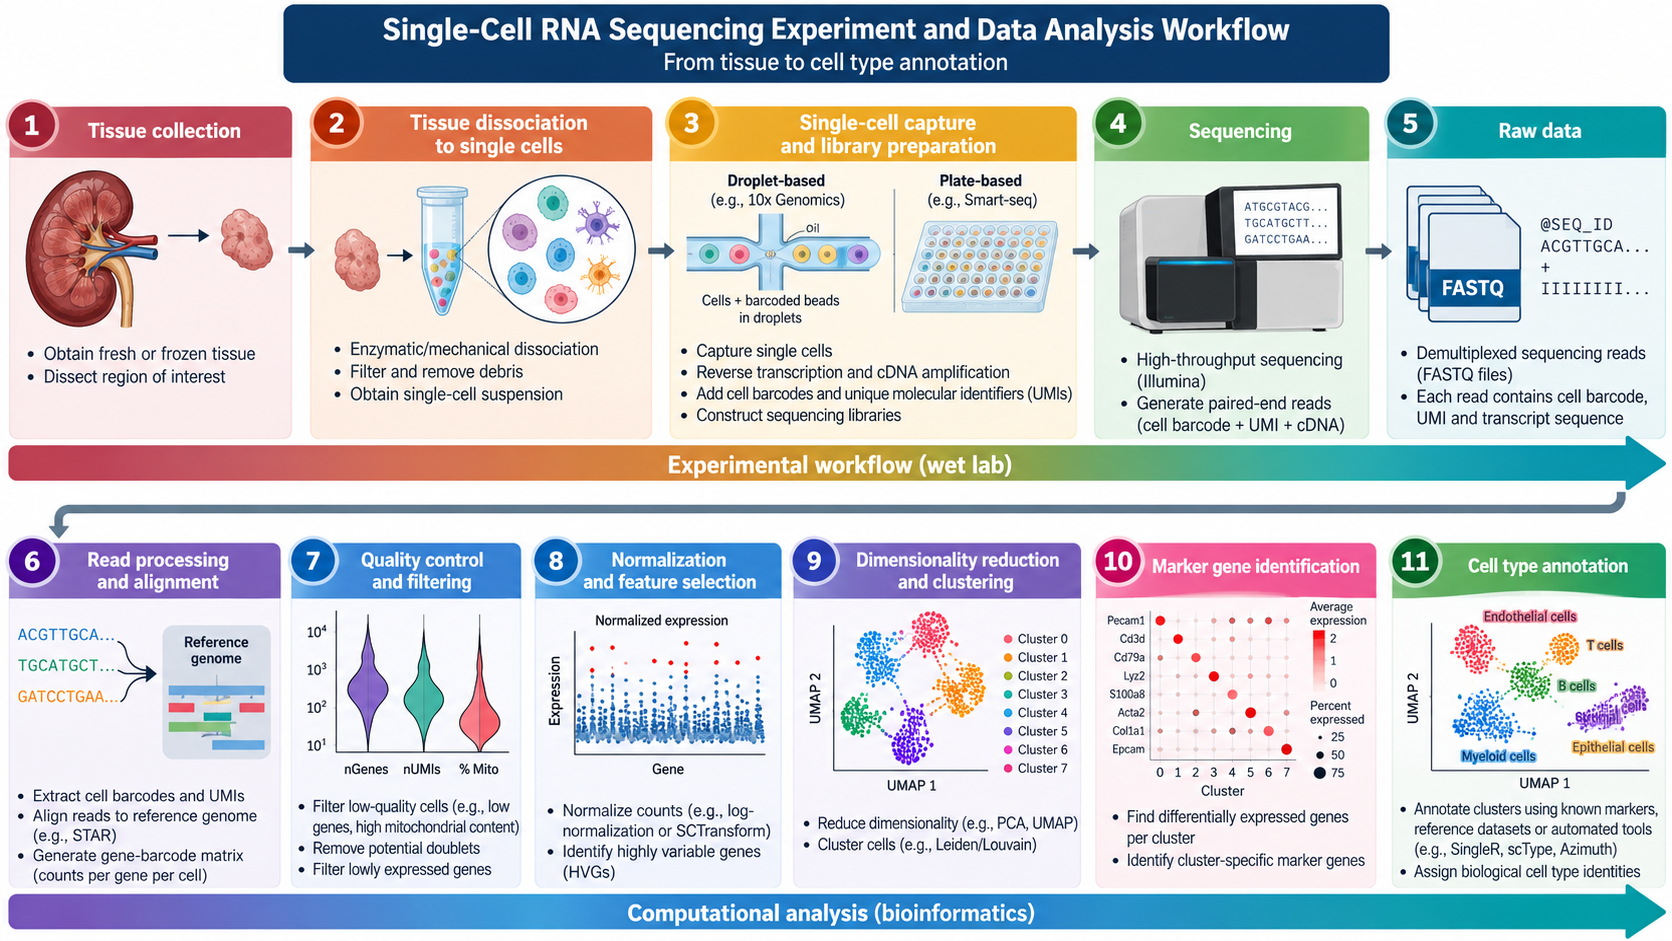
\includegraphics[width=\linewidth]{figures/ch06/ch06-01-v1-vague.png}};
\begin{scope}[x={(img.south east)},y={(img.north west)}]
  \tikzset{badmark/.style={draw=white,line width=0.8pt,fill=ChSixBad,text=white,circle,font=\sffamily\bfseries\scriptsize,inner sep=1.1pt,minimum size=4.2mm}}
  \node[badmark] at (0.09,0.74) {1};
  \node[badmark] at (0.36,0.80) {2};
  \node[badmark] at (0.91,0.78) {3};
  \node[badmark] at (0.24,0.36) {4};
  \node[badmark] at (0.55,0.36) {5};
  \node[badmark] at (0.91,0.28) {6};
\end{scope}
\end{tikzpicture}
\caption{First draft of a single-cell sequencing workflow diagram generated from a one-sentence prompt (teaching example of failure). Numbered problems: (1) top left draws a single kidney rather than lung tissue and shows only a single-sample path instead of parallel control and treated samples; (2) the wet-lab row omits cell-viability and library quality-control gates, mixes droplet-based (10x Genomics) and plate-based (Smart-seq) chemistries in panel 3, and leaves out sample pooling; (3) panel 5 frames the data product FASTQ as an operational step on par with sequencing; (4) panel 7 draws computational quality control as an ordinary inline panel with no pass or fail exits; (5) panel 9 collapses dimensionality reduction, neighbor-graph construction, clustering, and UMAP into a single panel without showing the fork from the neighbor graph to clustering versus visualization; (6) the endpoint lacks a feedback loop for anomalous clusters, the ``Stromal cells'' label collides directly with purple scatter points, and all text is baked into a non-editable bitmap.}\label{fig:ch06-01}
\end{figure}

When Dr.\ Chen zooms in to 200\% and checks the figure panel by panel against her Methods section, six flaws surface (Figure~\ref{fig:ch06-01}, red circles 1--6). First, panel 1 at the top left depicts a single kidney rather than lung tissue—because the prompt said only ``tissue''—and the entire diagram traces a single linear path, hiding where control and treated samples are processed separately and where they are pooled. Second, panel 3 crams droplet-based capture (10x Genomics) and plate-based sorting (Smart-seq) into the same step box while compressing cell capture, reverse transcription, cDNA amplification, and library construction into one black box, omitting both cell-viability and library quality-control gates. Third, panel 5 frames the data artifact ``Raw data (FASTQ)'' as an action step equivalent to ``Sequencing.'' Fourth, while panel 7 on the bottom row includes violin plots for quality-control filtering, it sits in a simple serial chain with no ``pass'' or ``fail'' branches. Fifth, panel 9 merges dimensionality reduction and clustering into a single UMAP scatter plot ringed by dashed ovals, obscuring the topology in which a $k$-nearest-neighbor ($k$-NN) graph built in principal-component space branches in parallel to graph clustering and to two-dimensional UMAP display. Sixth, the annotation endpoint in panel 11 lacks a return path for re-evaluating low-quality clusters or clustering resolution, stamps the label ``Stromal cells'' directly across a purple cluster, and locks heavy drop shadows, gradients, and dense text inside a non-editable bitmap.

A reviewer familiar with single-cell genomics would spot the contradictions between Figure 1A and the Methods text in five seconds. Yet when Dr.\ Chen spent the afternoon asking the chat interface to fix one panel at a time, repairing the organ icon scrambled the arrows, and fixing the arrows broke the layout. The solution developed in this chapter is straightforward: \textbf{translate your protocol into a structured step table first, draw the structural skeleton with a deterministic tool, and only then let AI generate the icons and visual styling.}

\section{What a Workflow Diagram Answers}

In a scientific paper, a method or experimental workflow diagram serves a different purpose from the mechanism figures discussed in Chapter 7. A mechanism diagram answers \emph{why} a phenomenon occurs—how molecules, cells, or components interact causally to produce an effect. A workflow diagram answers \textbf{how the research work was carried out step by step}: what operational steps were executed in the laboratory and on the computer, what material or data each step received and handed off, under what experimental parameters or quality-control criteria the process moved forward or looped back, and where parallel samples or computational branches diverged and converged.

Specifically, a clear workflow diagram must communicate four core elements:
\begin{enumerate}
\item \textbf{Steps (what operation is performed):} Concrete actions applied to biological specimens or datasets—such as ``Dissociation,'' ``Library construction,'' ``Alignment \& UMI counting,'' or ``Clustering (Leiden).'' Every step node should name a specific operation rather than a broad discipline.
\item \textbf{Products (what is produced and handed off):} The tangible material or data object generated at the end of one step and passed as input to the next—such as ``Single-cell suspension,'' ``Barcoded cDNA,'' ``FASTQ,'' or ``Filtered matrix.'' Placing product nodes at key transitions shows what crosses each boundary.
\item \textbf{Conditions and quality-control gates (when to proceed and when to return):} Experimental parameters and checkpoints governing whether the workflow continues along the main trunk. Any node marked as a quality-control (QC) check logically requires two exits: a forward ``Pass'' path and a ``Fail'' feedback path returning upstream to re-optimize digestion, rebuild a library, or adjust filtering thresholds.
\item \textbf{Branches and merges (what runs in parallel and where paths join):} Real workflows are rarely a single straight line. Control and treated samples are typically dissociated, captured, and converted into indexed libraries in parallel before pooling for sequencing; in computation, a principal-component neighbor graph forks into graph clustering and two-dimensional visualization. Where paths split and merge encodes the experimental and analytical logic.
\end{enumerate}

Once these four elements are defined, a strict boundary applies: \textbf{workflow arrows represent temporal sequence and material or data hand-off; they never represent biological causation, mechanism, or effect size.} In single-cell preparation, ``Dissociation $\rightarrow$ Single-cell suspension'' is a standard workflow relationship stating that an experimental operation yields a material product. By contrast, prior studies show that prolonged warm enzymatic dissociation can induce spurious expression of immediate-early stress-response genes in certain subpopulations (van den Brink et al., 2017). That observation is a biological effect or quality-control caveat triggered by handling. Drawing ``Dissociation $\rightarrow$ Stress-gene expression rises'' with the same solid workflow arrow conflates an operational step with an intracellular transcriptional response. Mechanistic caveats should instead be attached via a dotted callout line as a marginal note or stated in the caption.

So that readers never have to guess whether a box represents an action, a sample, or a quality check, this book uses a fixed visual grammar of nodes and arrows (Figure~\ref{fig:ch06-02}).

\begin{figure}[htbp]\centering
\resizebox{0.94\linewidth}{!}{% FIG ch06-02 flow grammar (English)%
% Shared styles for chapter 6 workflow TikZ figures.%
% Every figure inputs this file, so commands are defined with \providecommand.%
\providecolor{BookTeal}{HTML}{176C68}%
\providecolor{BookInk}{HTML}{23363E}%
\providecolor{BookRule}{HTML}{C8D6D6}%
\providecolor{BookPale}{HTML}{F1F6F5}%
\definecolor{WetPale}{HTML}{FBF1EA}%
\definecolor{Wet}{HTML}{B5653A}%
\definecolor{Seq}{HTML}{8A6D1F}%
\definecolor{DryPale}{HTML}{EEF4F7}%
\definecolor{Dry}{HTML}{2F6F8F}%
\definecolor{ChSixFeedback}{HTML}{7A8A90}%
\definecolor{ChSixBad}{HTML}{C0392B}%
\usetikzlibrary{arrows.meta,positioning,shapes.geometric,shapes.misc,fit,backgrounds,calc}%
\ifdefined\ChSixLayersReady\else%
  \pgfdeclarelayer{chsixlane}%
  \pgfsetlayers{chsixlane,background,main}%
  \def\ChSixLayersReady{}%
\fi%

\tikzset{%
  chsix/.style={font=\sffamily\scriptsize, text=BookInk, align=center},%
  flowstep/.style={%
    chsix, rounded corners=2pt, draw=Wet, line width=0.45pt, fill=white,%
    text width=19mm, minimum height=7.4mm, inner sep=1.3pt,%
  },%
  flowstepdry/.style={flowstep, draw=Dry},%
  flowstepseq/.style={flowstep, draw=Seq},%
  artifact/.style={%
    chsix, trapezium, trapezium left angle=70, trapezium right angle=110,%
    trapezium stretches=true,%
    draw=BookInk, line width=0.45pt, fill=white,%
    minimum height=6.2mm, inner sep=1.2pt,%
  },%
  gate/.style={%
    chsix, diamond, aspect=1.7, draw=BookInk, line width=0.45pt, fill=white,%
    text width=12mm, inner sep=0.6pt, minimum height=8mm,%
  },%
  opt/.style={flowstep, dashed, draw=BookInk!70},%
  optdry/.style={flowstepdry, dashed, draw=BookInk!70},%
  stack/.style={flowstep},%
  link/.style={-{Stealth[length=1.6mm]}, semithick, draw=BookInk},%
  linkthin/.style={-{Stealth[length=1.2mm]}, thin, draw=BookInk!80},%
  back/.style={-{Stealth[length=1.5mm]}, dashed, draw=ChSixFeedback},%
  conn/.style={%
    circle, draw=BookInk, line width=0.5pt, minimum size=4.6mm,%
    font=\sffamily\scriptsize\bfseries, inner sep=0pt, text=BookInk,%
  },%
  lanetitle/.style={font=\sffamily\bfseries\small, text=BookInk, align=left},%
  passlabel/.style={font=\sffamily\scriptsize, text=BookInk, fill=white, inner sep=0.7pt, align=center},%
  mergelabel/.style={font=\sffamily\scriptsize, text=BookInk, fill=white, inner sep=0.8pt, align=center},%
  taglab/.style={font=\sffamily\scriptsize, text=ChSixFeedback, fill=white, inner sep=0.8pt, align=center},%
  gramcap/.style={font=\sffamily\scriptsize, text=BookInk, align=left, anchor=west},%
}%

% Offset card behind a two-sample step. Text stays on the front node only.%
\providecommand{\ChSixCardBack}[1]{%
  \begin{pgfonlayer}{background}%
    \draw[Wet, line width=0.45pt, rounded corners=2pt, fill=white]%
      ([shift={(-0.55mm,0.55mm)}]#1.south west)%
      rectangle ([shift={(-0.55mm,0.55mm)}]#1.north east);%
  \end{pgfonlayer}%
}%
% #1 options, #2 name, #3 position (with parentheses), #4 text%
\providecommand{\ChSixCard}[4]{%
  \node[stack, #1] (#2) at #3 {#4};%
  \ChSixCardBack{#2}%
}%

\providecommand{\ChSixMaybeLabel}[1]{%
  \ifdefined\nolabels\else#1\fi%
}%

\providecommand{\ChSixIcon}[2]{%
  \ifdefined\ChSixShowIcons%
    \IfFileExists{#1}{%
      \node[anchor=south, inner sep=0] at ([yshift=0.7mm]#2.north)%
        {\includegraphics[height=5.4mm]{#1}};%
    }{}%
  \fi%
}%
%
\begin{tikzpicture}[x=1mm, y=1mm, font=\sffamily\scriptsize, text=BookInk]%
  \node[anchor=north west, font=\sffamily\bfseries\small] (titleL) at (0,0) {Node \& arrow grammar};%
  \draw[BookRule, line width=0.4pt] (0,-7) rectangle (128,-126);%

  \node[flowstep] (g1) at (16,-14) {Step};%
  \node[gramcap, text width=88mm] at (36,-14) {Rounded rectangle — what is done};%

  \node[artifact] (g2) at (16,-25) {Product};%
  \node[gramcap, text width=88mm] at (36,-25)%
    {Parallelogram — material or data handed to the next step};%

  \node[gate] (g3) at (16,-38) {QC};%
  \node[passlabel, anchor=west] at ([xshift=1.5mm]g3.east) {Pass};%
  \node[taglab, anchor=north west] at ([xshift=1.5mm, yshift=-0.6mm]g3.south east) {Fail};%
  \node[gramcap, text width=88mm] at (36,-38) {Diamond — two exits (pass / fail)};%

  \node[opt] (g4) at (16,-50) {Optional};%
  \node[gramcap, text width=88mm] at (36,-50) {Dashed rounded rectangle};%

  \node[stack] (gs1) at (13,-61) {};%
  \ChSixCardBack{gs1}%
  \node[stack] (gs2) at (16.2,-61) {Sample};%
  \node[gramcap, text width=88mm] at (36,-61) {Offset stack — done for each sample};%

  \draw[link] (6,-72) -- ++(16,0);%
  \node[gramcap, text width=88mm] at (36,-72) {Solid arrow — sequence \& hand-off};%

  \draw[back] (6,-83) to[out=20, in=160] (24,-83);%
  \node[gramcap, text width=88mm] at (36,-83) {Dashed arc — feedback / return};%

  \fill (16,-94) circle (0.7pt);%
  \node[gramcap, text width=88mm] at (36,-94) {Dot — branch / merge point};%

  \node[conn] (gc) at (16,-105) {A};%
  \node[gramcap, text width=88mm] at (36,-105) {Circle connector — continues elsewhere};%

  \fill[WetPale, draw=Wet, line width=0.3pt] (6,-116) rectangle (16,-122);%
  \fill[DryPale, draw=Dry, line width=0.3pt] (18,-116) rectangle (28,-122);%
  \node[gramcap, text width=88mm] at (36,-119) {Swim-lane fill — wet lab / computational};%

  \node[anchor=north west, font=\sffamily\bfseries\small] (titleR) at (0,-130) {Workflow $\neq$ causation};%
  \node[flowstep] (d1) at (20,-146) {Dissociation};%
  \node[artifact] (d2) at (52,-146) {Single-cell\\suspension};%
  \draw[link] (d1) -- (d2);%
  \node[gramcap] at (76,-146) {Workflow: sequence \& hand-off};%

  \node[flowstep] (e1) at (20,-164) {Dissociation};%
  \node[gramcap, text width=72mm] at (42,-164) {$\Rightarrow$ stress-gene expression rises};%
  \draw[BookInk!45, densely dotted] (e1.east) -- ++(6,0);%
  \node[gramcap, anchor=north west, text width=122mm] at (0,-176)%
    {Mechanistic claims belong in notes or captions, not workflow arrows (van den Brink et al.\ 2017).};%
\end{tikzpicture}%
}
\caption{Node and arrow conventions used for workflow diagrams in this book. Each shape has one meaning. Bottom panel: a workflow arrow means sequence and hand-off; mechanistic information such as dissociation-induced stress-gene expression (van den Brink et al., 2017) is written as an annotation, not drawn as a workflow arrow.}\label{fig:ch06-02}
\end{figure}

As illustrated in Figure~\ref{fig:ch06-02}, this grammar enforces a ``one shape, one meaning'' encoding principle (Wong, 2010; Wong, 2011a):
\begin{itemize}
\item \textbf{Rounded rectangles represent operational steps:} Labels inside rounded rectangles state the action performed (e.g., ``Dissociation,'' ``PCA'') without mixing in input or output file names.
\item \textbf{Parallelograms represent material or data products:} Placed at key hand-offs between steps or at branch endpoints, parallelograms identify the physical specimen or data object being transferred (e.g., ``Single-cell suspension,'' ``Raw count matrix'').
\item \textbf{Diamonds represent quality-control or decision gates:} Every diamond must display both a ``Pass'' exit and a ``Fail'' exit.
\item \textbf{Dashed rounded rectangles represent optional steps:} Used for protocol modules that depend on tissue properties, batch structure, or software choice (e.g., ``RBC lysis,'' ``Integration (optional)'').
\item \textbf{Offset stacked rounded rectangles represent per-sample parallel execution:} When control and treated samples undergo the exact same sequence of steps independently, drawing two slightly offset stacked cards communicates ``performed separately for each sample'' without duplicating an entire chain of boxes across the page.
\item \textbf{Solid arrows and dashed arcs distinguish forward hand-offs from feedback loops:} Uniform dark-slate solid arrows with triangular heads indicate forward sequence and hand-off; medium-grey dashed arcs indicate return loops when a QC gate fails or downstream inspection reveals anomalous results.
\item \textbf{Solid dots, circle connectors, and swim-lane fills organize macro-layout:} A small solid dot marks an explicit branch or merge point; a lettered circle connector (such as ``A'') links a path across rows or swim lanes; and pale warm (wet-lab and sequencing) versus pale cool (computational analysis) background bands paired with bold lane headers allow readers to separate bench work from computation even in grayscale print.
\end{itemize}

\section{From Methods Notes to a Step Table}

Why does pasting a draft Methods section into an AI tool almost always produce a flawed flowchart? Because prose in a Methods section is organized by \textbf{narrative economy}, whereas a workflow diagram must be organized by \textbf{input-to-product hand-offs}.

In written paragraphs, authors routinely group related techniques into a single clause, omit intermediate data objects that are obvious to specialists, or tuck conditional branches behind phrases such as ``subsequently,'' ``in parallel,'' or ``where appropriate.'' On a diagram canvas, however, every arrow must connect a specific source node to a specific target node, and every parallel track must split and rejoin at an exact coordinate. Consequently, the essential first step from laboratory notes to a method diagram is not picking a color palette or prompting an image model, but decomposing the prose into a structured \textbf{step table}.

We demonstrate this translation using our chapter's main case study: a droplet-based 3$'$ scRNA-seq workflow comparing lung tissue cellular composition between control and treated mice. Both the wet-lab procedures and computational pipeline follow established textbook and community best-practice conventions: droplet barcoding and unique molecular identifier (UMI) principles follow Islam et al.\ (2014), Macosko et al.\ (2015), Zheng et al.\ (2017), and Hwang et al.\ (2018); computational quality control, normalization, feature selection, dimensionality reduction, neighbor-graph construction, clustering, and annotation follow Wolf et al.\ (2018), Luecken and Theis (2019), and Heumos et al.\ (2023); Leiden community detection follows Traag et al.\ (2019); computational doublet detection and ambient RNA decontamination follow Wolock et al.\ (2019) and Young and Behjati (2020), respectively.

To maintain strict scientific integrity, we emphasize that the passage below is a \textbf{pedagogical methods record} written specifically for this book. Because it represents a generic protocol rather than measurements from a specific experiment, every empirical parameter—enzyme concentrations, digestion duration, strainer mesh size, viability cutoff, target cell recovery, and filtering thresholds—is explicitly marked as ``[author to fill in]'':

\begin{BookNote}
Lung tissues are harvested from one control mouse and one treated mouse and processed separately. Each tissue sample is minced and digested in [enzyme and concentration] at [temperature] for [duration] with gentle mechanical trituration, then passed through a [pore size] cell strainer, followed by [optional: red blood cell lysis; dead-cell removal]. Cell concentration and viability are measured by [method]; if viability falls below [threshold], the dissociation protocol is re-optimized. Qualifying single-cell suspensions are loaded onto a microfluidic chip at [target cell number] per channel to co-encapsulate individual cells with barcoded gel beads in water-in-oil droplets. Within each droplet, cells are lysed and polyadenylated mRNAs are reverse-transcribed using primers carrying a cell barcode, a UMI, and a poly(dT) tail. After emulsion breakage, barcoded cDNA is purified and amplified by PCR, and fragment size distribution is recorded. Sequencing libraries are constructed via enzymatic fragmentation, end repair, A-tailing, adapter ligation, and sample-index PCR. Following library fragment-size and concentration QC, the two indexed libraries are pooled at [ratio] and sequenced paired-end on [sequencing platform] (Read 1: cell barcode + UMI; Read 2: cDNA insert).

Raw sequencing reads are demultiplexed into FASTQ files, aligned to [reference genome build], and quantified by UMI counting to generate a raw gene $\times$ barcode count matrix for each sample. Cell-containing barcodes are called against background empty droplets, and low-quality cells are filtered out based on total UMI counts, detected gene counts, and mitochondrial read fraction using thresholds [determined by author from sample distributions], alongside optional doublet detection and ambient RNA correction. Filtered count matrices from the two samples are merged, normalized for library size, and log-transformed. Highly variable genes are selected for principal component analysis (PCA; with optional batch integration if batch effects are present), and a $k$-nearest-neighbor ($k$-NN) graph is constructed in principal-component space. The $k$-NN graph is partitioned into clusters using the Leiden algorithm and separately embedded into two dimensions with UMAP for visualization. Marker genes are identified for each cluster and combined with canonical markers and reference atlases to assign cell-type annotations; if low-quality clusters or inappropriate resolution are detected, analysis returns to refine cell QC thresholds or clustering resolution.
\end{BookNote}

A conversational AI assistant can help draft an initial table from this text—extracting candidate operations, highlighting implicit intermediate products, and pointing out where QC gates need failure paths. However, the author must enforce two non-negotiable rules during this step. First, \textbf{AI must never invent experimental parameters or quality-control thresholds.} When asked to summarize a protocol, large language models readily hallucinate plausible-sounding digestion temperatures, incubation times, cell viability percentages, or mitochondrial read cutoffs. Every parameter slot must remain marked as ``pending confirmation'' until the author fills it in directly from laboratory notebooks and analysis scripts. Second, \textbf{each step must occupy its own row with an explicit ID, swim lane, input, product, key conditions, QC or branching logic, and downstream target ID.} Table~\ref{tab:ch06-01} shows the verified step table, which serves as the single source of truth for constructing and auditing every version of the figure in this chapter.

\begin{table}[htbp]\centering\tiny
\setlength{\tabcolsep}{2pt}
\renewcommand{\arraystretch}{1.05}
\caption{Step table for the droplet-based single-cell RNA-seq experimental and computational workflow (the single source of truth for drawing and verification).}\label{tab:ch06-01}
\begin{tabularx}{\linewidth}{@{}l>{\raggedright\arraybackslash}p{15mm}l>{\raggedright\arraybackslash}p{16mm}>{\raggedright\arraybackslash}p{16mm}YYl@{}}
\toprule
\textbf{ID} & \textbf{Step} & \textbf{Lane} & \textbf{Input} & \textbf{Product} & \textbf{Key conditions (author fills in)} & \textbf{QC / decision \& optional branches} & \textbf{Next} \\
\midrule
W1 & Tissue collection & Wet & Mice (control, treated) & Fresh lung tissue & Sampling time, medium & Separate per sample & W2 \\
W2 & Dissociation & Wet & Lung tissue & Crude suspension & Enzyme, conc., temp., time & Separate per sample & W3 \\
W3 & Filtering \& washing & Wet & Crude suspension & Single-cell suspension & Strainer pore size & Opt.\ W3a RBC lysis, W3b dead-cell removal & Q1 \\
Q1 & Count \& viability & Wet & Single-cell suspension & Viability record & Assay, viability cutoff & Pass $\rightarrow$ W4; Fail $\rightarrow$ W2 (dashed arc) & W4 \\
W4 & Droplet capture & Wet & Suspension, beads, oil & Droplets ($\approx$1 cell + 1 bead) & Target cell count, chip & Separate channel per sample & W5 \\
W5 & RT \& cDNA amp. & Wet & Droplets & Barcoded cDNA & PCR cycle number & Fragment profile recorded (no branch) & W6 \\
W6 & Library construction & Wet & Barcoded cDNA & Indexed library & Frag., adapters, index PCR & Separate index per sample & Q2 \\
Q2 & Library QC & Wet & Indexed library & Size \& conc.\ record & Assay, pass criteria & Pass $\rightarrow$ S1; Fail $\rightarrow$ W6 & S1 \\
S1 & Pooling \& sequencing & Wet (seq.) & \textbf{Both sample libraries} (merge) & Raw reads $\rightarrow$ FASTQ & Platform, read length, depth & Handed via connector A to comp.\ lane & C1 \\
C1 & Alignment \& UMI count & Comp. & FASTQ, reference build & Raw count matrix (per sample) & Software version, reference & Quantified per sample & C2 \\
C2 & Cell calling & Comp. & Raw count matrix & Cell barcodes & Calling method & Separates cells from empty droplets & Q3 \\
Q3 & Cell QC & Comp. & Cell matrix & Filtered matrix & UMI, gene, mito.\ cutoffs & Parallel opt.: C3a doublet $\parallel$ C3b ambient RNA & C4 \\
C4 & Merge \& normalize & Comp. & \textbf{Both filtered matrices} (merge) & Normalized matrix & Normalization method & Two sample matrices merge here & C5 \\
C5 & Highly variable genes & Comp. & Normalized matrix & HVG list & Gene count & — & C6 \\
C6 & PCA & Comp. & HVG expression & PC coordinates & Number of PCs & Opt.\ C6a batch integration (dashed) & C7 \\
C7 & $k$-NN graph & Comp. & PC coordinates & Neighbor graph & $k$ value & \textbf{Fork} $\rightarrow$ C8 and C9 & C8, C9 \\
C8 & Clustering (Leiden) & Comp. & Neighbor graph & Cluster labels & Resolution & — & C10 \\
C9 & UMAP & Comp. & Neighbor graph & 2D coords (\textbf{display only}) & Embedding parameters & Terminal display; not linked to C8/C11 & (Display) \\
C10 & Marker genes & Comp. & Norm.\ matrix + clusters & Marker gene table & Statistical test & — & C11 \\
C11 & Cell-type annotation & Comp. & Markers, reference atlas & Annotated cell atlas & Reference version & Poor clusters/resolution $\rightarrow$ Q3 or C8 & End \\
\bottomrule
\end{tabularx}
\end{table}

Examining Table~\ref{tab:ch06-01} closely shows how building a step table resolves five methodological subtleties before any drawing begins:
\begin{enumerate}
\item \textbf{Two distinct merge points across the two lanes:} In the wet-lab lane, the control and treated samples are handled independently from tissue collection (W1) through library quality control (Q2), ligated with distinct sample indices, and physically pooled for the first time at S1 (Pooling \& sequencing). In the computational lane, demultiplexed FASTQ files are again processed per sample through alignment and UMI counting (C1), cell calling (C2), and cell-level QC (Q3), merging for the second time only at C4 (Merge \& normalize).
\item \textbf{In-droplet reverse transcription versus post-breakage cDNA amplification:} In standard 3$'$ droplet protocols, cell lysis and mRNA reverse transcription occur inside intact water-in-oil droplets, whereas bulk PCR amplification of cDNA takes place after breaking the emulsion and purifying the first-strand product. Because minor procedural details vary across kit chemistries, Table~\ref{tab:ch06-01} groups ``in-droplet RT, emulsion breakage, and cDNA amplification'' into step W5 so the diagram stays accurate across chemistry revisions.
\item \textbf{Idealized droplet iconography versus computational denoising:} Visual icons for step W4 conventionally depict the idealized target state—one cell paired with one barcoded gel bead inside a droplet. In actual microfluidic loading under Poisson statistics, most droplets contain no cell (capturing only ambient cell-free RNA from the suspension buffer) and a small fraction encapsulate two or more cells (doublets). Recognizing this physical reality explains why the computational lane requires empty-droplet cell calling (C2) as well as optional doublet detection (C3a) and ambient RNA correction (C3b).
\item \textbf{Optional modules and software-dependent integration placement:} Different single-cell toolkits place multi-sample batch integration at different stages—some operate on normalized expression matrices or feature sets, whereas methods such as Harmony adjust principal-component embeddings directly. Table~\ref{tab:ch06-01} places integration (C6a) as a dashed optional box under PCA (C6) and pairs doublet detection (C3a) and ambient RNA correction (C3b) as parallel optional branches under Q3, noting that the figure caption must state this simplification.
\item \textbf{The parallel fork at C7:} Constructing the $k$-NN graph (C7) produces the shared topological representation from which both Leiden community clustering (C8) and UMAP two-dimensional embedding (C9) branch out. C9 terminates at the display coordinates product and has no arrow pointing into C8 or C11. If an author visually inspects marker expression overlaid on UMAP coordinates during manual curation, that practice should be described in the caption (``UMAP is used for display and visual inspection'') rather than drawn as a computational dependency arrow.
\end{enumerate}

Once the candidate step table is drafted, the author must verify every row against experimental records and analysis scripts using the nine-point confirmation checklist in Table~\ref{tab:ch06-02}. Any optional step that was not actually performed in the study (for example, if neither red blood cell lysis nor dead-cell removal was used) should be deleted from a manuscript figure rather than left as a speculative dashed box.

\begin{table}[htbp]\centering\footnotesize
\setlength{\tabcolsep}{4pt}
\renewcommand{\arraystretch}{1.12}
\caption{Author confirmation checklist (to be verified item by item against lab notebooks and code after AI drafts the step table).}\label{tab:ch06-02}
\begin{tabularx}{\linewidth}{@{}c>{\raggedright\arraybackslash}p{30mm}Y@{}}
\toprule
\textbf{No.} & \textbf{Verification dimension} & \textbf{Specific question the author must confirm from experimental records or analysis scripts} \\
\midrule
1 & Batch \& chip channels & Were the two samples processed in the same batch on separate channels of the same microfluidic chip? (Determines whether optional integration box C6a is needed.) \\
2 & Optional wet-lab steps & Were W3a (RBC lysis) and W3b (dead-cell removal) actually performed? Delete dashed boxes for any step not performed rather than leaving ``possibly done.'' \\
3 & Wet-lab QC actions & What were the exact pass criteria at Q1 and Q2, and what action was taken on failure (re-optimize dissociation, re-sample, or terminate)? \\
4 & Sequencing read structure & Do the sequencing platform and paired-end read structure (what sequences reside in Read 1 vs.\ Read 2) match the chemistry manual? \\
5 & Alignment \& reference build & What exact software name, version, reference genome assembly, and gene annotation release were used in C1? \\
6 & Cell QC \& denoising & Were the three Q3 filtering thresholds set from sample distributions and applied per sample, and were C3a and C3b actually executed? \\
7 & Clustering space & Was the neighbor graph for C8 clustering built in PCA (or integrated latent) space rather than on 2D UMAP coordinates? \\
8 & Annotation basis & What marker gene lists and reference datasets were used in C11, and was manual expert curation performed? \\
9 & Table-to-figure closure & Does every box in the diagram map to a row in Table~\ref{tab:ch06-01}, and is every row either drawn or explicitly declared as omitted in the caption? \\
\bottomrule
\end{tabularx}
\end{table}

\section{Structure First: Drawing the Skeleton with Deterministic Tools}

Once Table~\ref{tab:ch06-01} has been verified, why not feed the table directly into an image-generation model to render the complete diagram?

Because \textbf{image-generation models optimize for pixel-level visual plausibility, not graph-theoretical accuracy}; they cannot guarantee that the number of nodes, the direction of arrows, or the exact branch and merge junctions will match your specification. And in a workflow diagram, a single structural error—an arrow pointing the wrong way or a missing QC exit—is fatal. The reliable strategy is \emph{structure first}: use a deterministic drawing tool (such as TikZ, PowerPoint, draw.io, or Adobe Illustrator—any tool where boxes and connectors snap to exact coordinates) to translate Table~\ref{tab:ch06-01} directly into a \textbf{structural skeleton} (Figure~\ref{fig:ch06-03}).

\begin{figure}[htbp]\centering
\resizebox{\linewidth}{!}{% FIG ch06-03 skeleton (English)%
% Shared styles for chapter 6 workflow TikZ figures.%
% Every figure inputs this file, so commands are defined with \providecommand.%
\providecolor{BookTeal}{HTML}{176C68}%
\providecolor{BookInk}{HTML}{23363E}%
\providecolor{BookRule}{HTML}{C8D6D6}%
\providecolor{BookPale}{HTML}{F1F6F5}%
\definecolor{WetPale}{HTML}{FBF1EA}%
\definecolor{Wet}{HTML}{B5653A}%
\definecolor{Seq}{HTML}{8A6D1F}%
\definecolor{DryPale}{HTML}{EEF4F7}%
\definecolor{Dry}{HTML}{2F6F8F}%
\definecolor{ChSixFeedback}{HTML}{7A8A90}%
\definecolor{ChSixBad}{HTML}{C0392B}%
\usetikzlibrary{arrows.meta,positioning,shapes.geometric,shapes.misc,fit,backgrounds,calc}%
\ifdefined\ChSixLayersReady\else%
  \pgfdeclarelayer{chsixlane}%
  \pgfsetlayers{chsixlane,background,main}%
  \def\ChSixLayersReady{}%
\fi%

\tikzset{%
  chsix/.style={font=\sffamily\scriptsize, text=BookInk, align=center},%
  flowstep/.style={%
    chsix, rounded corners=2pt, draw=Wet, line width=0.45pt, fill=white,%
    text width=19mm, minimum height=7.4mm, inner sep=1.3pt,%
  },%
  flowstepdry/.style={flowstep, draw=Dry},%
  flowstepseq/.style={flowstep, draw=Seq},%
  artifact/.style={%
    chsix, trapezium, trapezium left angle=70, trapezium right angle=110,%
    trapezium stretches=true,%
    draw=BookInk, line width=0.45pt, fill=white,%
    minimum height=6.2mm, inner sep=1.2pt,%
  },%
  gate/.style={%
    chsix, diamond, aspect=1.7, draw=BookInk, line width=0.45pt, fill=white,%
    text width=12mm, inner sep=0.6pt, minimum height=8mm,%
  },%
  opt/.style={flowstep, dashed, draw=BookInk!70},%
  optdry/.style={flowstepdry, dashed, draw=BookInk!70},%
  stack/.style={flowstep},%
  link/.style={-{Stealth[length=1.6mm]}, semithick, draw=BookInk},%
  linkthin/.style={-{Stealth[length=1.2mm]}, thin, draw=BookInk!80},%
  back/.style={-{Stealth[length=1.5mm]}, dashed, draw=ChSixFeedback},%
  conn/.style={%
    circle, draw=BookInk, line width=0.5pt, minimum size=4.6mm,%
    font=\sffamily\scriptsize\bfseries, inner sep=0pt, text=BookInk,%
  },%
  lanetitle/.style={font=\sffamily\bfseries\small, text=BookInk, align=left},%
  passlabel/.style={font=\sffamily\scriptsize, text=BookInk, fill=white, inner sep=0.7pt, align=center},%
  mergelabel/.style={font=\sffamily\scriptsize, text=BookInk, fill=white, inner sep=0.8pt, align=center},%
  taglab/.style={font=\sffamily\scriptsize, text=ChSixFeedback, fill=white, inner sep=0.8pt, align=center},%
  gramcap/.style={font=\sffamily\scriptsize, text=BookInk, align=left, anchor=west},%
}%

% Offset card behind a two-sample step. Text stays on the front node only.%
\providecommand{\ChSixCardBack}[1]{%
  \begin{pgfonlayer}{background}%
    \draw[Wet, line width=0.45pt, rounded corners=2pt, fill=white]%
      ([shift={(-0.55mm,0.55mm)}]#1.south west)%
      rectangle ([shift={(-0.55mm,0.55mm)}]#1.north east);%
  \end{pgfonlayer}%
}%
% #1 options, #2 name, #3 position (with parentheses), #4 text%
\providecommand{\ChSixCard}[4]{%
  \node[stack, #1] (#2) at #3 {#4};%
  \ChSixCardBack{#2}%
}%

\providecommand{\ChSixMaybeLabel}[1]{%
  \ifdefined\nolabels\else#1\fi%
}%

\providecommand{\ChSixIcon}[2]{%
  \ifdefined\ChSixShowIcons%
    \IfFileExists{#1}{%
      \node[anchor=south, inner sep=0] at ([yshift=0.7mm]#2.north)%
        {\includegraphics[height=5.4mm]{#1}};%
    }{}%
  \fi%
}%
%
% English node labels for FIG ch06-03 / ch06-06%
\providecommand{\ChSixLaneWet}{Wet lab \& sequencing}%
\providecommand{\ChSixLaneDry}{Computational analysis}%
\providecommand{\ChSixTxtWone}{Tissue\\collection}%
\providecommand{\ChSixTxtWtwo}{Dissociation}%
\providecommand{\ChSixTxtWthree}{Filtering\\\& washing}%
\providecommand{\ChSixTxtWthreeA}{RBC lysis}%
\providecommand{\ChSixTxtWthreeB}{Dead-cell\\removal}%
\providecommand{\ChSixTxtQone}{Count \&\\viability}%
\providecommand{\ChSixTxtWfour}{Droplet capture\\\& barcoding}%
\providecommand{\ChSixTxtWfive}{RT \& cDNA\\amplification}%
\providecommand{\ChSixTxtWsix}{Library\\construction}%
\providecommand{\ChSixTxtQtwo}{Library\\QC}%
\providecommand{\ChSixTxtSone}{Pooling \&\\sequencing}%
\providecommand{\ChSixTxtCone}{Alignment \&\\UMI counting}%
\providecommand{\ChSixTxtCtwo}{Cell calling}%
\providecommand{\ChSixTxtQthree}{Cell QC}%
\providecommand{\ChSixTxtCthreeA}{Doublet\\detection}%
\providecommand{\ChSixTxtCthreeB}{Ambient RNA\\correction}%
\providecommand{\ChSixTxtCfour}{Merge \&\\normalize}%
\providecommand{\ChSixTxtCfive}{Highly\\variable genes}%
\providecommand{\ChSixTxtCsix}{PCA}%
\providecommand{\ChSixTxtCsixA}{Integration\\(optional)}%
\providecommand{\ChSixTxtCseven}{k-NN graph}%
\providecommand{\ChSixTxtCeight}{Clustering\\(Leiden)}%
\providecommand{\ChSixTxtCnine}{UMAP}%
\providecommand{\ChSixTxtCten}{Marker\\genes}%
\providecommand{\ChSixTxtCeleven}{Cell-type\\annotation}%
\providecommand{\ChSixArtSusp}{Single-cell\\suspension}%
\providecommand{\ChSixArtCdna}{Barcoded\\cDNA}%
\providecommand{\ChSixArtLib}{Sequencing\\library}%
\providecommand{\ChSixArtFastq}{FASTQ}%
\providecommand{\ChSixArtRaw}{Raw count\\matrix}%
\providecommand{\ChSixArtFilt}{Filtered\\matrix}%
\providecommand{\ChSixArtAtlas}{Annotated\\cell atlas}%
\providecommand{\ChSixArtUmap}{UMAP coordinates\\(display only)}%
\providecommand{\ChSixQoneFail}{Fail: optimise\\dissociation}%
\providecommand{\ChSixQtwoFail}{Fail}%
\providecommand{\ChSixCelevenFail}{Low-quality clusters\\or poor resolution}%
\providecommand{\ChSixMergeNote}{Two samples merge here}%
\providecommand{\ChSixPass}{Pass}%
%
\begin{tikzpicture}[x=1cm,y=1cm]%
  % Row positions are set with relative anchors in ch06-workflow-draw.tex%
% so Chinese and English labels do not share one set of fixed centres.%
%
  % Workflow structure (FIG ch06-03 skeleton / ch06-06 final).%
% Requires ch06-styles and a label file. Nodes are placed from the node%
% above them so wrapped English labels cannot land on the next row.%
\coordinate (origin) at (0,0);%
% Final figures carry icons above the nodes; keep feedback arcs above them.%
\ifdefined\ChSixShowIcons
  \def\ChSixLift{6.6mm}%
  \def\ChSixArc{12.2mm}%
\else
  \def\ChSixLift{0mm}%
  \def\ChSixArc{8.4mm}%
\fi

% ----- Wet lab, row 1: collection through droplet capture -----%
\ChSixCard{anchor=north west}{nW1}{(origin)}{\ChSixMaybeLabel{\ChSixTxtWone}}%
\ChSixCard{anchor=west}{nW2}{([xshift=3.2mm]nW1.east)}{\ChSixMaybeLabel{\ChSixTxtWtwo}}%
\ChSixCard{anchor=west}{nW3}{([xshift=3.2mm]nW2.east)}{\ChSixMaybeLabel{\ChSixTxtWthree}}%
\node[gate, anchor=west] (nQ1) at ([xshift=3.6mm]nW3.east) {\ChSixMaybeLabel{\ChSixTxtQone}};%
\ChSixCard{anchor=west}{nW4}{([xshift=6.4mm]nQ1.east)}{\ChSixMaybeLabel{\ChSixTxtWfour}}%

\draw[link] (nW1) -- (nW2);%
\draw[link] (nW2) -- (nW3);%
\draw[link] (nW3) -- (nQ1);%
\draw[link] (nQ1) -- (nW4);%

\coordinate (arcQ1) at ($(nW2.north)!0.5!(nQ1.north)+(0,\ChSixArc)$);%
\draw[back] ([yshift=\ChSixLift]nQ1.north) -- ([yshift=\ChSixLift]nQ1.north |- arcQ1) -- ([yshift=\ChSixLift]nW2.north |- arcQ1) -- ([yshift=\ChSixLift]nW2.north);%
\node[taglab, anchor=south] (q1fail) at (arcQ1) {\ChSixMaybeLabel{\ChSixQoneFail}};%
\node[passlabel] (passQ1) at ($(nQ1.east)!0.5!(nW4.west)+(0,1.3mm)$) {\ChSixMaybeLabel{\ChSixPass}};%

\node[lanetitle, anchor=south west] (laneWet) at ([yshift=1.2mm]q1fail.north -| origin) {\ChSixMaybeLabel{\ChSixLaneWet}};%

% Optional lysis / dead-cell removal under filtering, product to their right.%
\node[opt, anchor=north] (nW3a) at ([yshift=-2.2mm]nW3.south) {\ChSixMaybeLabel{\ChSixTxtWthreeA}};%
\node[opt, anchor=north] (nW3b) at ([yshift=-1.8mm]nW3a.south) {\ChSixMaybeLabel{\ChSixTxtWthreeB}};%
\draw[linkthin] (nW3.south) -- (nW3a.north);%
\draw[linkthin] (nW3a.south) -- (nW3b.north);%
\node[artifact, anchor=north west] (aSusp) at ([xshift=3.2mm, yshift=-2.2mm]nW3.south east) {\ChSixMaybeLabel{\ChSixArtSusp}};%

% ----- Wet lab, row 2 (left-aligned; FASTQ is the hand-off into connector A) -----%
\ChSixCard{anchor=north west}{nW5}{([yshift=-10mm]nW3b.south -| nW1.west)}{\ChSixMaybeLabel{\ChSixTxtWfive}}%
\ChSixCard{anchor=west}{nW6}{([xshift=2.4mm]nW5.east)}{\ChSixMaybeLabel{\ChSixTxtWsix}}%
\node[gate, anchor=west] (nQ2) at ([xshift=2.4mm]nW6.east) {\ChSixMaybeLabel{\ChSixTxtQtwo}};%
\node[flowstepseq, anchor=west] (nS1) at ([xshift=6.2mm]nQ2.east) {\ChSixMaybeLabel{\ChSixTxtSone}};%
\node[artifact, anchor=west] (aFastq) at ([xshift=2.2mm]nS1.east) {\ChSixMaybeLabel{\ChSixArtFastq}};%
\node[conn, anchor=west] (nA) at ([xshift=2mm]aFastq.east) {A};%

\draw[link] (nW5) -- (nW6);%
\draw[link] (nW6) -- (nQ2);%
\draw[link] (nQ2) -- (nS1);%
\draw[link] (nS1) -- (aFastq);%
\draw[link] (aFastq) -- (nA);%
\node[passlabel] (passQ2) at ($(nQ2.east)!0.5!(nS1.west)+(0,1.3mm)$) {\ChSixMaybeLabel{\ChSixPass}};%

\coordinate (arcQ2) at ($(nW6.north)!0.5!(nQ2.north)+(0,\ChSixArc)$);%
\draw[back] ([yshift=\ChSixLift]nQ2.north) -- ([yshift=\ChSixLift]nQ2.north |- arcQ2) -- ([yshift=\ChSixLift]nW6.north |- arcQ2) -- ([yshift=\ChSixLift]nW6.north);%
\node[taglab, anchor=south] (q2fail) at (arcQ2) {\ChSixMaybeLabel{\ChSixQtwoFail}};%

\node[artifact, anchor=north] (aCdna) at ([yshift=-2mm]$(nW5.south)!0.5!(nW6.south)$) {\ChSixMaybeLabel{\ChSixArtCdna}};%
\node[artifact, anchor=north] (aLib) at ([yshift=-2mm]$(nW6.south)!0.5!(nQ2.south)$) {\ChSixMaybeLabel{\ChSixArtLib}};%

% ----- Computational lane -----%
\node[conn, anchor=north west] (nA2) at ([yshift=-7mm]aCdna.south -| origin) {A};%
\node[flowstepdry, anchor=west] (nC1) at ([xshift=3.2mm]nA2.east) {\ChSixMaybeLabel{\ChSixTxtCone}};%
\node[flowstepdry, anchor=west] (nC2) at ([xshift=3.6mm]nC1.east) {\ChSixMaybeLabel{\ChSixTxtCtwo}};%
\node[gate, anchor=west] (nQ3) at ([xshift=4.2mm]nC2.east) {\ChSixMaybeLabel{\ChSixTxtQthree}};%
\node[flowstepdry, anchor=west] (nC4) at ([xshift=4.2mm]nQ3.east) {\ChSixMaybeLabel{\ChSixTxtCfour}};%
\node[flowstepdry, anchor=west] (nC5) at ([xshift=3.6mm]nC4.east) {\ChSixMaybeLabel{\ChSixTxtCfive}};%

\draw[link] (nA2) -- (nC1);%
\draw[link] (nC1) -- (nC2);%
\draw[link] (nC2) -- (nQ3);%
\draw[link] (nQ3) -- (nC4);%
\draw[link] (nC4) -- (nC5);%

\node[mergelabel, anchor=south] (mergeNote) at ([yshift=1mm]nC4.north) {\ChSixMaybeLabel{\ChSixMergeNote}};%

\coordinate (arcDry) at ($(nC1.north)!0.5!(nQ3.north)+(0,\ChSixArc)$);%
\node[taglab, anchor=south, text width=28mm] (c11fail) at (arcDry) {\ChSixMaybeLabel{\ChSixCelevenFail}};%
\node[lanetitle, anchor=south west] (laneDry) at ([yshift=1.2mm]c11fail.north -| origin) {\ChSixMaybeLabel{\ChSixLaneDry}};%

% Optional doublet / ambient RNA under the cell-QC gate.%
\node[optdry, anchor=north east] (nC3a) at ([yshift=-2mm, xshift=-1mm]nQ3.south) {\ChSixMaybeLabel{\ChSixTxtCthreeA}};%
\node[optdry, anchor=north west] (nC3b) at ([yshift=-2mm, xshift=1mm]nQ3.south) {\ChSixMaybeLabel{\ChSixTxtCthreeB}};%
\draw[linkthin] (nQ3.south) -- (nC3a.north);%
\draw[linkthin] (nQ3.south) -- (nC3b.north);%
\draw[linkthin] (nC3a.south) -- ++(0,-2.4mm) -| (nC3b.south);%

\node[artifact, anchor=north] (aRaw) at ([yshift=-2mm]$(nC1.south)!0.5!(nC2.south)$) {\ChSixMaybeLabel{\ChSixArtRaw}};%
\node[artifact, anchor=north] (aFilt) at ([yshift=-2mm]nC4.south) {\ChSixMaybeLabel{\ChSixArtFilt}};%

% Fork: k-NN graph splits to clustering (continues) and UMAP (display only).%
\node[flowstepdry, anchor=north west] (nC6) at ([yshift=-4mm]aRaw.south -| nC1.west) {\ChSixMaybeLabel{\ChSixTxtCsix}};%
\node[flowstepdry, anchor=west] (nC7) at ([xshift=4mm]nC6.east) {\ChSixMaybeLabel{\ChSixTxtCseven}};%
\node[flowstepdry, anchor=west] (nC8) at ([xshift=5mm]nC7.east) {\ChSixMaybeLabel{\ChSixTxtCeight}};%
\node[flowstepdry, anchor=west] (nC10) at ([xshift=3.6mm]nC8.east) {\ChSixMaybeLabel{\ChSixTxtCten}};%
\node[flowstepdry, anchor=west] (nC11) at ([xshift=3.6mm]nC10.east) {\ChSixMaybeLabel{\ChSixTxtCeleven}};%
\node[optdry, anchor=north] (nC6a) at ([yshift=-2mm]nC6.south) {\ChSixMaybeLabel{\ChSixTxtCsixA}};%
\node[flowstepdry, anchor=north] (nC9) at ([yshift=-3.2mm]nC7.south) {\ChSixMaybeLabel{\ChSixTxtCnine}};%
\node[artifact, anchor=north, text width=22mm] (aUmap) at ([yshift=-1.8mm]nC9.south) {\ChSixMaybeLabel{\ChSixArtUmap}};%
\node[artifact, anchor=north] (aAtlas) at ([yshift=-2mm]$(nC10.south)!0.5!(nC11.south)$) {\ChSixMaybeLabel{\ChSixArtAtlas}};%

\draw[link] (nC5.south) -- ++(0,-2.5mm) -| (nC6.north);%
\draw[linkthin] (nC6.south) -- (nC6a.north);%
\draw[link] (nC6) -- (nC7);%
\draw[link] (nC7) -- (nC8);%
\draw[link] (nC8) -- (nC10);%
\draw[link] (nC10) -- (nC11);%
\draw[link] (nC7.south) -- (nC9.north);%

% Return from annotation to clustering, and the long return to cell QC.%
\coordinate (bus) at ([yshift=-4.5mm]aUmap.south);%
\draw[back] (nC11.south) -- (nC11.south |- bus) -- (nC8.south |- bus) -- (nC8.south);%
\draw[back] (nC11.east) -- ++(3.2mm,0) |- (c11fail.east);%
\draw[back] (c11fail.west) -| ([yshift=\ChSixLift]nQ3.north);%

% Connector A joins the lanes in the gutter between them.%
\draw[link] (nA.south) -- ++(0,-2.2mm) -| (nA2.north);%

\ChSixIcon{figures/ch06/icons/ch06-icon-01.png}{nW1}%
\ChSixIcon{figures/ch06/icons/ch06-icon-02.png}{nW2}%
\ChSixIcon{figures/ch06/icons/ch06-icon-03.png}{nW3}%
\ChSixIcon{figures/ch06/icons/ch06-icon-04.png}{nQ1}%
\ChSixIcon{figures/ch06/icons/ch06-icon-05.png}{nW4}%
\ChSixIcon{figures/ch06/icons/ch06-icon-06.png}{nW5}%
\ChSixIcon{figures/ch06/icons/ch06-icon-07.png}{nW6}%
\ChSixIcon{figures/ch06/icons/ch06-icon-08.png}{nS1}%
\ChSixIcon{figures/ch06/icons/ch06-icon-09.png}{nC1}%
\ChSixIcon{figures/ch06/icons/ch06-icon-10.png}{nC2}%
\ChSixIcon{figures/ch06/icons/ch06-icon-11.png}{nC7}%
\ChSixIcon{figures/ch06/icons/ch06-icon-12.png}{nC11}%

\begin{pgfonlayer}{chsixlane}%
  \node[rectangle, fit=(laneWet)(nW1)(nW4)(nW3b)(aSusp)(nA)(aCdna)(aLib)(q1fail),%
        fill=WetPale, draw=none, inner sep=1.1mm] {};%
  \node[rectangle, fit=(laneDry)(nA2)(nC5)(nC11)(nC6a)(aUmap)(aAtlas)(c11fail)(nC3a)(nC3b),%
        fill=DryPale, draw=none, inner sep=1.1mm] {};%
\end{pgfonlayer}%
%
\end{tikzpicture}%
}
\caption{Workflow structure drawn directly from the step table (skeleton). Each box corresponds to one row of Table~\ref{tab:ch06-01}. Stacked boxes are performed separately for each of the two samples, which are pooled at sequencing; their count matrices are merged before normalization. Diamonds are QC gates, dashed arcs return to earlier steps on failure, and dashed boxes are optional steps. Clustering and UMAP both branch from the $k$-NN graph.}\label{fig:ch06-03}
\end{figure}

Comparing Figure~\ref{fig:ch06-03} row by row against Table~\ref{tab:ch06-01} shows how a deterministic skeleton locks in all topological constraints at once:
\begin{itemize}
\item \textbf{Two horizontal swim lanes and a cross-lane connector:} The upper warm swim lane (``Wet lab \& sequencing'') contains 9 primary nodes (W1--W6, Q1, Q2, S1) and 2 optional dashed boxes (W3a ``RBC lysis,'' W3b ``Dead-cell removal''). The lower cool swim lane (``Computational analysis'') contains 11 primary nodes (C1--C11, Q3) and 3 optional dashed boxes (C3a ``Doublet detection,'' C3b ``Ambient RNA correction,'' C6a ``Integration (optional)''). After S1 outputs ``FASTQ,'' circle connector ``A'' bridges the gutter to connector ``A'' before C1.
\item \textbf{Per-sample parallel tracks and two merge points:} Steps W1--W6 use offset double-card stacks to show control and treated lung tissues processed independently until converging into the single deep-amber box S1 (``Pooling \& sequencing''). In the computational lane, a bold note above C4 (``Merge \& normalize'') states ``Two samples merge here,'' marking where per-sample filtered matrices combine.
\item \textbf{Eight product parallelograms at critical hand-offs:} Rather than placing a product box between every pair of steps—which adds clutter without insight (Wong, 2011a)—parallelograms appear selectively where specimens or data undergo major transformations: ``Single-cell suspension,'' ``Barcoded cDNA,'' ``Sequencing library,'' ``FASTQ,'' ``Raw count matrix,'' ``Filtered matrix,'' ``Annotated cell atlas,'' and ``UMAP coordinates (display only).''
\item \textbf{Three quality-control gates and four feedback arcs:} Diamonds Q1 and Q2 send forward ``Pass'' arrows along the main axis and route upward dashed ``Fail'' arcs back to W2 (``Fail: optimise dissociation'') and W6 (``Fail''). At the computational endpoint C11 (``Cell-type annotation''), two dashed feedback arcs route back to Q3 (``Cell QC'') and C8 (``Clustering (Leiden)'') when ``Low-quality clusters or poor resolution'' are found.
\end{itemize}

Crucially, Figure~\ref{fig:ch06-03} is already a complete workflow diagram ready for journal submission. Bringing AI in after this step serves only to add recognizable step icons so readers can scan the workflow faster. If you want to explore layout variations using \textbf{sketch mode} in the \scidraw{} drawing workspace (\sdtool{ai-drawing}), you can export a label-free PNG of this skeleton as a sketch input alongside a style prompt. Keep in mind, however, an essential platform fact: \textbf{a sketch provides a layout reference, not a structural lock.} Image-generation models do not guarantee that every node, branch, and arrowhead in an uploaded sketch will be preserved one-to-one.

\section{Common Structural Errors and How to Fix Them}

When reviewing method diagrams in manuscripts, four structural errors appear repeatedly. Figure~\ref{fig:ch06-04} pairs each incorrect drawing (marked with a red cross) against its corrected topology (marked with a green checkmark), accompanied by a revision instruction for manual or AI-assisted editing.

\begin{figure}[htbp]\centering
\resizebox{0.90\linewidth}{!}{% FIG ch06-04 structure errors (English)%
% Shared styles for chapter 6 workflow TikZ figures.%
% Every figure inputs this file, so commands are defined with \providecommand.%
\providecolor{BookTeal}{HTML}{176C68}%
\providecolor{BookInk}{HTML}{23363E}%
\providecolor{BookRule}{HTML}{C8D6D6}%
\providecolor{BookPale}{HTML}{F1F6F5}%
\definecolor{WetPale}{HTML}{FBF1EA}%
\definecolor{Wet}{HTML}{B5653A}%
\definecolor{Seq}{HTML}{8A6D1F}%
\definecolor{DryPale}{HTML}{EEF4F7}%
\definecolor{Dry}{HTML}{2F6F8F}%
\definecolor{ChSixFeedback}{HTML}{7A8A90}%
\definecolor{ChSixBad}{HTML}{C0392B}%
\usetikzlibrary{arrows.meta,positioning,shapes.geometric,shapes.misc,fit,backgrounds,calc}%
\ifdefined\ChSixLayersReady\else%
  \pgfdeclarelayer{chsixlane}%
  \pgfsetlayers{chsixlane,background,main}%
  \def\ChSixLayersReady{}%
\fi%

\tikzset{%
  chsix/.style={font=\sffamily\scriptsize, text=BookInk, align=center},%
  flowstep/.style={%
    chsix, rounded corners=2pt, draw=Wet, line width=0.45pt, fill=white,%
    text width=19mm, minimum height=7.4mm, inner sep=1.3pt,%
  },%
  flowstepdry/.style={flowstep, draw=Dry},%
  flowstepseq/.style={flowstep, draw=Seq},%
  artifact/.style={%
    chsix, trapezium, trapezium left angle=70, trapezium right angle=110,%
    trapezium stretches=true,%
    draw=BookInk, line width=0.45pt, fill=white,%
    minimum height=6.2mm, inner sep=1.2pt,%
  },%
  gate/.style={%
    chsix, diamond, aspect=1.7, draw=BookInk, line width=0.45pt, fill=white,%
    text width=12mm, inner sep=0.6pt, minimum height=8mm,%
  },%
  opt/.style={flowstep, dashed, draw=BookInk!70},%
  optdry/.style={flowstepdry, dashed, draw=BookInk!70},%
  stack/.style={flowstep},%
  link/.style={-{Stealth[length=1.6mm]}, semithick, draw=BookInk},%
  linkthin/.style={-{Stealth[length=1.2mm]}, thin, draw=BookInk!80},%
  back/.style={-{Stealth[length=1.5mm]}, dashed, draw=ChSixFeedback},%
  conn/.style={%
    circle, draw=BookInk, line width=0.5pt, minimum size=4.6mm,%
    font=\sffamily\scriptsize\bfseries, inner sep=0pt, text=BookInk,%
  },%
  lanetitle/.style={font=\sffamily\bfseries\small, text=BookInk, align=left},%
  passlabel/.style={font=\sffamily\scriptsize, text=BookInk, fill=white, inner sep=0.7pt, align=center},%
  mergelabel/.style={font=\sffamily\scriptsize, text=BookInk, fill=white, inner sep=0.8pt, align=center},%
  taglab/.style={font=\sffamily\scriptsize, text=ChSixFeedback, fill=white, inner sep=0.8pt, align=center},%
  gramcap/.style={font=\sffamily\scriptsize, text=BookInk, align=left, anchor=west},%
}%

% Offset card behind a two-sample step. Text stays on the front node only.%
\providecommand{\ChSixCardBack}[1]{%
  \begin{pgfonlayer}{background}%
    \draw[Wet, line width=0.45pt, rounded corners=2pt, fill=white]%
      ([shift={(-0.55mm,0.55mm)}]#1.south west)%
      rectangle ([shift={(-0.55mm,0.55mm)}]#1.north east);%
  \end{pgfonlayer}%
}%
% #1 options, #2 name, #3 position (with parentheses), #4 text%
\providecommand{\ChSixCard}[4]{%
  \node[stack, #1] (#2) at #3 {#4};%
  \ChSixCardBack{#2}%
}%

\providecommand{\ChSixMaybeLabel}[1]{%
  \ifdefined\nolabels\else#1\fi%
}%

\providecommand{\ChSixIcon}[2]{%
  \ifdefined\ChSixShowIcons%
    \IfFileExists{#1}{%
      \node[anchor=south, inner sep=0] at ([yshift=0.7mm]#2.north)%
        {\includegraphics[height=5.4mm]{#1}};%
    }{}%
  \fi%
}%
%
\begin{tikzpicture}[x=1mm, y=1mm, font=\sffamily\scriptsize, text=BookInk]%
  \tikzset{%
    onestep/.style={flowstep, minimum height=6.5mm},%
    onedry/.style={flowstepdry, minimum height=6.5mm},%
    oneseq/.style={flowstepseq, minimum height=6.5mm},%
    twostep/.style={flowstep, minimum height=8.4mm},%
    twoseq/.style={flowstepseq, minimum height=8.4mm},%
    prod/.style={artifact, minimum height=6.5mm},%
  }%
  % (a)%
  \node[anchor=north west, font=\sffamily\bfseries] (aH) at (0,0)%
    {(a)\ Visualization drawn upstream of analysis};%
  \node[onedry, anchor=north west] (a1b)%
    at ([xshift=11mm, yshift=-1.5mm]aH.south west) {k-NN graph};%
  \node[onedry, anchor=west] (a2b) at ([xshift=6mm]a1b.east) {UMAP};%
  \node[onedry, anchor=west] (a3b) at ([xshift=6mm]a2b.east) {Clustering};%
  \node[onedry, anchor=west] (a4b) at ([xshift=6mm]a3b.east) {Annotation};%
  \draw[link] (a1b) -- (a2b) -- (a3b) -- (a4b);%
  \node[anchor=east, font=\sffamily\bfseries, text=ChSixBad]%
    at ([xshift=-4mm]a1b.west) {\bookcross};%

  \node[onedry, anchor=north west] (a1g) at ([yshift=-2.6mm]a1b.south west) {k-NN graph};%
  \node[onedry, anchor=west] (a2g) at ([xshift=6mm]a1g.east) {Clustering};%
  \node[onedry, anchor=west] (a3g) at ([xshift=6mm]a2g.east) {Annotation};%
  \node[onedry, anchor=north] (a4g) at ([yshift=-3.2mm]a1g.south) {UMAP};%
  \node[prod, anchor=west] (a5g) at ([xshift=6mm]a4g.east) {Display only};%
  \draw[link] (a1g) -- (a2g) -- (a3g);%
  \draw[link] (a1g.south) -- (a4g.north);%
  \draw[link] (a4g) -- (a5g);%
  \coordinate (aGmid) at ($(a1g.north)!0.5!(a4g.south)$);%
  \coordinate (aMark) at (a1g.west |- aGmid);%
  \node[anchor=east, font=\sffamily\bfseries, text=BookTeal]%
    at ([xshift=-4mm]aMark) {\bookcheck};%
  \coordinate (aNoteAt) at (a4g.south -| 0,0);%
  \node[anchor=north west, text width=120mm, text=BookInk!75] (aNote)%
    at ([yshift=-1.5mm]aNoteAt)%
    {Make UMAP a parallel branch from the k-NN graph, not linked to clustering or annotation};%

  % (b)%
  \node[anchor=north west, font=\sffamily\bfseries] (bH)%
    at ([yshift=-1.8mm]aNote.south west) {(b)\ Step and product in one box};%
  \node[onedry, anchor=north west, text width=42mm] (b1)%
    at ([xshift=11mm, yshift=-1.5mm]bH.south west)%
    {FASTQ $\rightarrow$ align $\rightarrow$ matrix};%
  \node[anchor=east, font=\sffamily\bfseries, text=ChSixBad]%
    at ([xshift=-4mm]b1.west) {\bookcross};%

  \node[prod, anchor=north west, minimum width=16mm] (b2a)%
    at ([yshift=-2.8mm]b1.south west) {FASTQ};%
  \node[onedry, anchor=west, text width=32mm] (b2b)%
    at ([xshift=6.5mm]b2a.east) {Align \& UMI count};%
  \node[prod, anchor=west, text width=30mm] (b2c)%
    at ([xshift=6.5mm]b2b.east) {Raw count matrix};%
  \draw[link] (b2a) -- (b2b);%
  \draw[link] (b2b) -- (b2c);%
  \node[anchor=east, font=\sffamily\bfseries, text=BookTeal]%
    at ([xshift=-4mm]b2a.west) {\bookcheck};%
  \coordinate (bNoteAt) at (b2b.south -| 0,0);%
  \node[anchor=north west, text width=120mm, text=BookInk!75] (bNote)%
    at ([yshift=-1.5mm]bNoteAt)%
    {Separate step boxes and product parallelograms so each hand-off is visible};%

  % (c)%
  \node[anchor=north west, font=\sffamily\bfseries] (cH)%
    at ([yshift=-1.8mm]bNote.south west) {(c)\ QC gate with no exit};%
  \node[onestep, anchor=north west, text width=26mm] (c1b)%
    at ([xshift=11mm, yshift=-1.5mm]cH.south west) {Dissociation};%
  \node[onestep, anchor=west, text width=30mm] (c2b)%
    at ([xshift=6mm]c1b.east) {Viability check};%
  \node[onestep, anchor=west, text width=20mm] (c3b)%
    at ([xshift=6mm]c2b.east) {Loading};%
  \draw[link] (c1b) -- (c2b) -- (c3b);%
  \node[anchor=east, font=\sffamily\bfseries, text=ChSixBad]%
    at ([xshift=-4mm]c1b.west) {\bookcross};%

  \node[onestep, anchor=north west, text width=26mm] (c1g)%
    at ([yshift=-3.6mm]c1b.south west) {Dissociation};%
  \node[gate, anchor=west, text width=15mm, minimum height=9mm, aspect=1.6] (c2g)%
    at ([xshift=6.5mm]c1g.east) {Viability};%
  \node[onestep, anchor=west, text width=20mm] (c3g)%
    at ([xshift=13mm]c2g.east) {Loading};%
  \draw[link] (c1g) -- (c2g);%
  \draw[link] (c2g) -- (c3g);%
  \node[passlabel, anchor=south] (cPass)%
    at ([yshift=1.8mm]$(c2g.east)!0.5!(c3g.west)$) {Pass};%
  \coordinate (cBase) at ($(c1g.south)!0.5!(c2g.south)+(0,-3.8mm)$);%
  \draw[back, rounded corners=1.6mm] (c2g.south) -- (c2g.south |- cBase)%
    -- (c1g.south |- cBase) -- (c1g.south);%
  \node[taglab, anchor=north] (cFailLab) at ([yshift=-1.2mm]cBase) {Fail};%
  \coordinate (cMid) at ($(c2g.north)!0.5!(cFailLab.south)$);%
  \coordinate (cMark) at (c1g.west |- cMid);%
  \node[anchor=east, font=\sffamily\bfseries, text=BookTeal]%
    at ([xshift=-4mm]cMark) {\bookcheck};%
  \coordinate (cNoteAt) at (cFailLab.south -| 0,0);%
  \node[anchor=north west, text width=120mm, text=BookInk!75] (cNote)%
    at ([yshift=-1.5mm]cNoteAt)%
    {Use a diamond with a fail arc back to the earlier step};%

  % (d)%
  \node[anchor=north west, font=\sffamily\bfseries] (dH)%
    at ([yshift=-1.8mm]cNote.south west) {(d)\ Parallel samples drawn in series};%
  \node[twostep, anchor=north west, text width=28mm] (d1b)%
    at ([xshift=11mm, yshift=-1.5mm]dH.south west) {Sample 1\\dissociation};%
  \node[twostep, anchor=west, text width=28mm] (d2b)%
    at ([xshift=6mm]d1b.east) {Sample 2\\dissociation};%
  \node[twoseq, anchor=west, text width=24mm] (d3b)%
    at ([xshift=6mm]d2b.east) {Sequencing};%
  \draw[link] (d1b) -- (d2b) -- (d3b);%
  \node[anchor=east, font=\sffamily\bfseries, text=ChSixBad]%
    at ([xshift=-4mm]d1b.west) {\bookcross};%

  \node[twostep, anchor=north west, text width=40mm] (d1g)%
    at ([yshift=-2.6mm]d1b.south west) {Sample 1:\\dissociation $\rightarrow$ library};%
  \node[twostep, anchor=north west, text width=40mm] (d2g)%
    at ([yshift=-1.8mm]d1g.south west) {Sample 2:\\dissociation $\rightarrow$ library};%
  \coordinate (dJoin) at ([xshift=7mm]$(d1g.east)!0.5!(d2g.east)$);%
  \node[twoseq, anchor=west, text width=26mm] (d3g)%
    at ([xshift=5.5mm]dJoin) {Pool \& sequence};%
  \draw[link] (d1g.east) -- (d1g.east -| dJoin);%
  \draw[link] (d2g.east) -- (d2g.east -| dJoin);%
  \draw[BookInk, semithick] (d1g.east -| dJoin) -- (d2g.east -| dJoin);%
  \fill[BookInk] (dJoin) circle (0.7pt);%
  \draw[link] (dJoin) -- (d3g.west);%
  \coordinate (dMid) at ($(d1g.north)!0.5!(d2g.south)$);%
  \coordinate (dMark) at (d1g.west |- dMid);%
  \node[anchor=east, font=\sffamily\bfseries, text=BookTeal]%
    at ([xshift=-4mm]dMark) {\bookcheck};%
  \coordinate (dNoteAt) at (d2g.south -| 0,0);%
  \node[anchor=north west, text width=120mm, text=BookInk!75]%
    at ([yshift=-1.5mm]dNoteAt)%
    {Draw samples in parallel and join at a merge point before sequencing};%
\end{tikzpicture}%
}
\caption{Four common structural errors in workflow diagrams and their corrections. (a) UMAP is a visual embedding; clustering is usually performed on the neighbor graph in principal-component space, so the two are parallel branches. (b) Drawing steps and products separately makes each hand-off visible. (c) A QC gate needs both a pass and a fail exit. (d) Samples processed separately are drawn in parallel and joined at a merge point.}\label{fig:ch06-04}
\end{figure}

\begin{enumerate}
\item \textbf{Visualization drawn upstream of analysis (Figure~\ref{fig:ch06-04}a):} A common mistake in single-cell figures is chaining ``$k$-NN graph $\rightarrow$ UMAP $\rightarrow$ Clustering $\rightarrow$ Annotation,'' implying that cells are clustered on 2D UMAP coordinates. Because non-linear 2D embeddings distort local and global distances when compressing high-dimensional data, standard pipelines typically run graph clustering (such as the Leiden algorithm) directly on the $k$-NN graph built in principal-component or batch-integrated space, while UMAP branches off the same $k$-NN graph solely for display (Luecken \& Theis, 2019; Traag et al., 2019; Heumos et al., 2023). \emph{Revision instruction: Make UMAP a parallel branch from the $k$-NN graph ending at a ``Display only'' product node, not connected to clustering or annotation.}
\item \textbf{Step and product combined in one box (Figure~\ref{fig:ch06-04}b):} Packing nouns and verbs into a single hybrid label such as ``FASTQ align matrix'' obscures what enters, what operation runs, and what is output. Separating the input parallelogram ``FASTQ,'' the step rectangle ``Align \& UMI count,'' and the output parallelogram ``Raw count matrix'' makes every hand-off explicit. \emph{Revision instruction: Separate step boxes and product parallelograms as ``input product $\rightarrow$ operational step $\rightarrow$ output product.''}
\item \textbf{QC gate with no exit (Figure~\ref{fig:ch06-04}c):} Drawing ``Viability check'' as an inline rectangle between ``Dissociation'' and ``Loading'' implies unconditional loading regardless of cell death. Replacing the rectangle with a diamond ``Viability'' gate with a forward ``Pass'' arrow to ``Loading'' and a dashed ``Fail'' arc returning to ``Dissociation'' restores the decision structure. \emph{Revision instruction: Replace the inline check box with a diamond QC gate showing both a forward ``Pass'' exit and a dashed ``Fail'' return arc.}
\item \textbf{Parallel samples drawn in series (Figure~\ref{fig:ch06-04}d):} Chaining ``Sample 1 dissociation $\rightarrow$ Sample 2 dissociation $\rightarrow$ Sequencing'' literally states that Sample 1 is dissociated into Sample 2. Drawing ``Sample 1: dissociation $\rightarrow$ library'' and ``Sample 2: dissociation $\rightarrow$ library'' in parallel converging at a merge dot before ``Pool \& sequence'' (or using offset stacked cards, as in Figure~\ref{fig:ch06-03}) accurately depicts parallel handling. \emph{Revision instruction: Draw independent samples on parallel branches that join at a merge point before pooling and sequencing.}
\end{enumerate}

\section{Letting AI Handle Icons and Visual Style}

To test whether a comprehensive written brief can compel an image-generation model to produce an accurate end-to-end flowchart without deterministic scaffolding, we ran a full-diagram generation experiment (V2). In the prompt below, we explicitly specified the two horizontal swim lanes, the icon inside each of the 9 upper-lane and 11 lower-lane nodes, the offset two-card stacks across steps 1--8 merging into the sequencer at step 9, the three dashed return arcs, the neighbor-graph fork into clustering versus 2D embedding, and strict flat-vector, text-free constraints:

\begin{Prompt}
A clean, flat, vector-style scientific workflow diagram on a pure white background,
landscape 16:9. Two horizontal swim lanes separated by a thin light-grey line.
Top lane (very light warm beige background): a left-to-right sequence of nine small
rounded-rectangle steps, each with one simple icon inside: (1) pink soft tissue on a dish,
(2) conical tube with tiny enzyme droplets, (3) cell strainer mesh over a tube,
(4) diamond checkpoint with counting grid and round cells, (5) microfluidic chip forming
droplets holding one cell and one bead, (6) small PCR tube, (7) short dsDNA fragments
with coloured end caps, (8) diamond checkpoint with fragment-size curve, (9) benchtop
sequencer box. Steps 1-8 drawn as stacks of two offset cards, merging into step 9.
Dashed curved arrows return from checkpoint 4 to step 2, and from checkpoint 8 to step 7.
Circle connector at right end of top lane and left end of bottom lane.
Bottom lane (very light cool blue-grey background): monitor with aligned reads, grid
matrix of squares, diamond checkpoint with filter funnel (two optional dashed boxes above
it joined back in), bar normalisation symbol, highlighted rows list, PCA scatter with two
axes arrows, network graph of dots and edges; from the network the path splits into upper
branch (coloured point clusters -> marker heatmap -> final cluster map with blank tag
shapes) and lower branch (2D point embedding, stops there). Dashed arrow returns from
final map to checkpoint. Warm orange-brown accents top, muted teal-blue bottom, dark slate
arrows. No text, no letters, no numbers, no labels, no 3D, no gradients, no shadows.
\end{Prompt}

We ran this exact prompt twice. In the first generation attempt, the model cropped the canvas into a narrow panoramic strip (roughly 2.5:1 aspect ratio) and drew arrowheads on \emph{both} ends of the bottom dashed return arc, turning what should be a one-way feedback loop from the final cluster map to the QC checkpoint into a bidirectional arrow. A second generation run restored the 16:9 aspect ratio and single-headed feedback arcs (Figure~\ref{fig:ch06-05}).

\begin{figure}[htbp]\centering
\begin{tikzpicture}
\definecolor{ChSixBad}{HTML}{C0392B}
\definecolor{ChSixGood}{HTML}{176C68}
\node[anchor=south west,inner sep=0] (img) at (0,0) {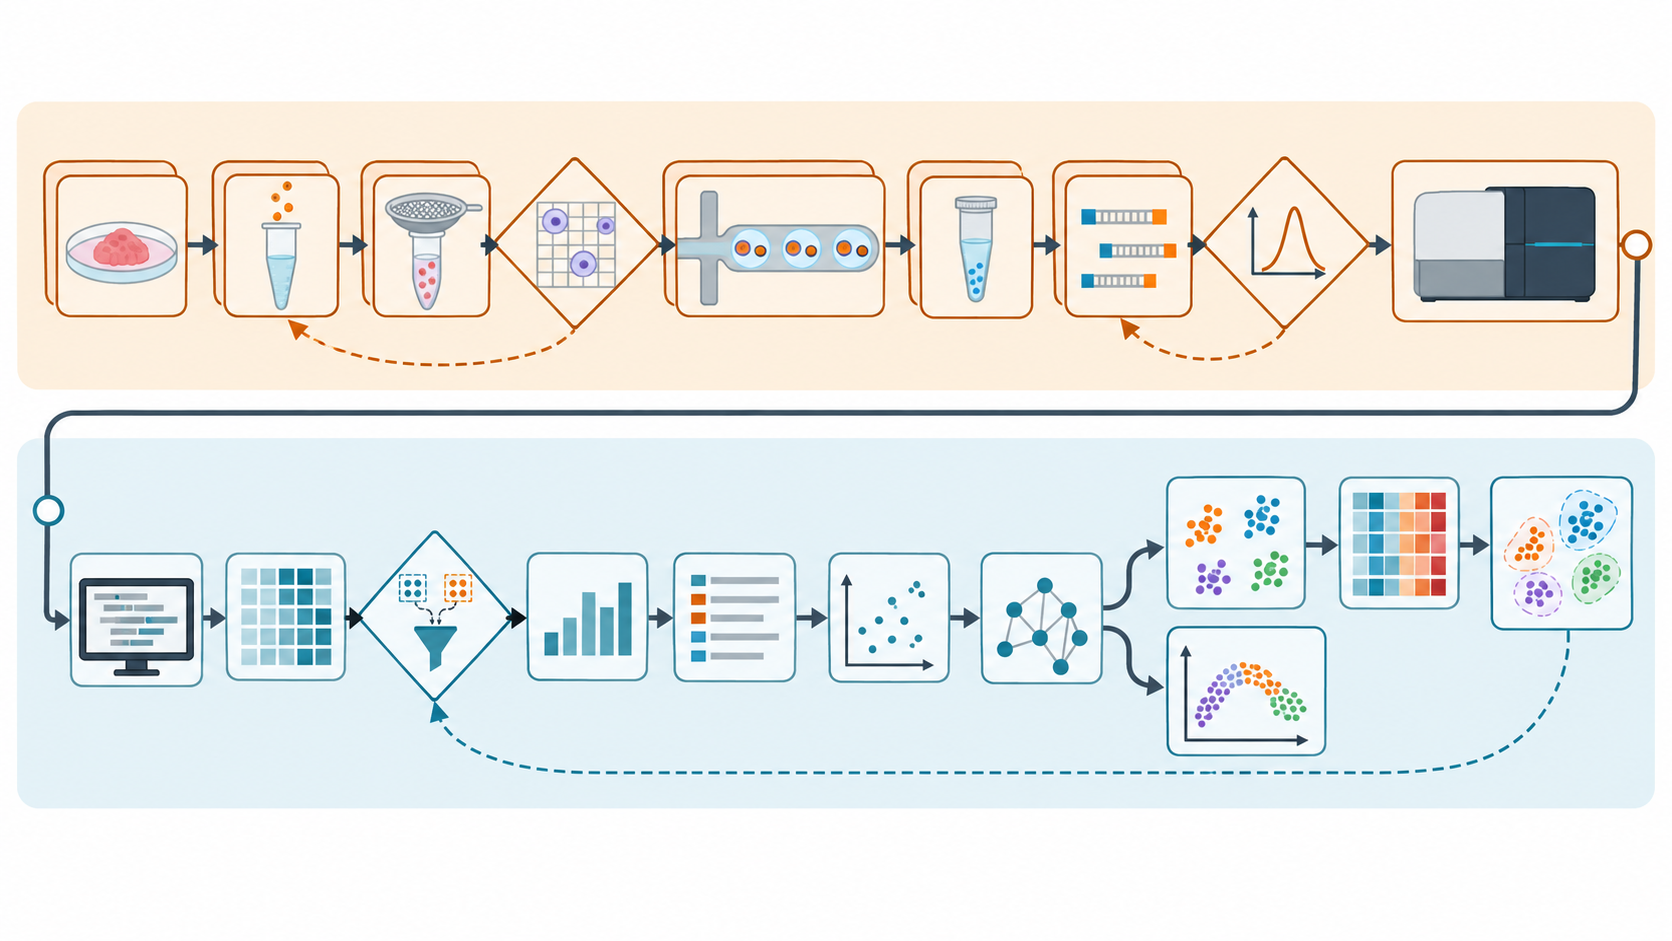
\includegraphics[width=\linewidth]{figures/ch06/ch06-05-v2-brief.png}};
\begin{scope}[x={(img.south east)},y={(img.north west)}]
  \tikzset{
    okmark/.style={draw=white,line width=0.6pt,fill=ChSixGood,text=white,circle,font=\sffamily\bfseries\tiny,inner sep=0.6pt,minimum size=3.6mm},
    ngmark/.style={draw=white,line width=0.6pt,fill=ChSixBad,text=white,circle,font=\sffamily\bfseries\tiny,inner sep=0.6pt,minimum size=3.6mm}
  }
  \node[okmark] at (0.07,0.85) {$\checkmark$};
  \node[okmark] at (0.16,0.85) {$\checkmark$};
  \node[okmark] at (0.25,0.85) {$\checkmark$};
  \node[ngmark] at (0.34,0.86) {$\times$};
  \node[okmark] at (0.25,0.60) {$\checkmark$};
  \node[okmark] at (0.46,0.85) {$\checkmark$};
  \node[okmark] at (0.58,0.85) {$\checkmark$};
  \node[okmark] at (0.67,0.85) {$\checkmark$};
  \node[ngmark] at (0.77,0.86) {$\times$};
  \node[okmark] at (0.72,0.61) {$\checkmark$};
  \node[ngmark] at (0.83,0.77) {$\times$};
  \node[ngmark] at (0.98,0.79) {$\times$};
  \node[okmark] at (0.08,0.44) {$\checkmark$};
  \node[okmark] at (0.17,0.44) {$\checkmark$};
  \node[ngmark] at (0.26,0.47) {$\times$};
  \node[ngmark] at (0.35,0.44) {$\times$};
  \node[okmark] at (0.44,0.44) {$\checkmark$};
  \node[okmark] at (0.53,0.44) {$\checkmark$};
  \node[okmark] at (0.62,0.44) {$\checkmark$};
  \node[okmark] at (0.68,0.42) {$\checkmark$};
  \node[okmark] at (0.68,0.25) {$\checkmark$};
  \node[okmark] at (0.84,0.52) {$\checkmark$};
  \node[ngmark] at (0.93,0.52) {$\times$};
  \node[okmark] at (0.58,0.14) {$\checkmark$};
\end{scope}
\end{tikzpicture}
\caption{A text-free workflow base image generated from the full brief, audited item by item against the step table. Green checkmarks ($\checkmark$) indicate nodes and arrows that match the specification; red crosses ($\times$) mark structural omissions or errors. Although the model preserved the neighbor-graph fork and the three specified feedback arcs, seven structural discrepancies remain across the diamond card stacks, the two sample merge points, the cross-lane hand-off arrow, the optional box placement, and the endpoint tag shapes; consequently, the final figure uses an author-drawn structure with model-generated icons only.}\label{fig:ch06-05}
\end{figure}

Printing Table~\ref{tab:ch06-01} and auditing Figure~\ref{fig:ch06-05} node by node and arrow by arrow shows both the strengths and the limits of full-diagram generation. On the positive side, the model obeyed the ``no text'' constraint, rendered all 20 primary step icons in left-to-right order, split the path after the 7th computational node ($k$-NN network graph) into an upper clustering branch and a lower 2D embedding branch that stops without rejoining, and drew the three specified return arcs (Q1 $\rightarrow$ W2, Q2 $\rightarrow$ W6, and C11 $\rightarrow$ Q3) in the right direction. Nevertheless, the seven red crosses in Figure~\ref{fig:ch06-05} expose structural defects that prevent using the image as a workflow backbone:
\begin{enumerate}
\item \textbf{Incomplete two-sample card stacks (top row, 4th and 8th nodes):} Although the prompt requested two offset cards for steps 1--8, only the six rounded-rectangle steps received double cards; both diamond checkpoints (Q1 and Q2) were drawn as single-layer diamonds.
\item \textbf{Missing sample merge junctions (before the sequencer and at the 4th bottom node):} Only a single arrow connects the library QC diamond to the sequencer, omitting the pooling of two sample libraries; similarly, the normalization node on the bottom row shows no convergence of two filtered matrices.
\item \textbf{Ambiguous cross-lane connector hand-off (top right):} The upper circle connector sits directly against the sequencer border without a distinct hand-off arrow and leaves no space for the ``FASTQ'' product parallelogram.
\item \textbf{Misplaced optional boxes (bottom row, 3rd node):} Instead of placing the two dashed optional boxes (C3a and C3b) above the cell-QC diamond, the model shrank them into tiny dotted squares stuffed \emph{inside} the diamond alongside the filter funnel, leaving no room for text labels.
\item \textbf{Endpoint and icon detail discrepancies (bottom right):} The final cluster map at C11 surrounds the point clusters with dashed outlines rather than blank rounded tag shapes; the PCR tube at step 6 is elongated like a centrifuge tube, and subtle gradients and 3D perspective remain on several vessels.
\end{enumerate}

The V2 experiment demonstrates a clear trade-off: generating a full workflow diagram as a single bitmap can suggest a color palette and icon style, but auditing and fixing its topology takes more effort than drawing a deterministic skeleton—and every regeneration forces you to re-audit all twenty-plus nodes and arrows from scratch.

A cleaner division of labor is the \textbf{icon-sheet workflow (V3)}. Instead of asking the image generator to draw swim lanes and arrows, we generate 12 isolated, style-matched icons on a $4 \times 3$ white grid, slice them into transparent PNGs, and place them onto the deterministic skeleton of Figure~\ref{fig:ch06-03}. In \scidraw{}, an author can enter from the workflow diagram generator (\sdtool{workflow-diagram-generator}) or take the ``Mechanism \& Workflow'' route in the figure workflow wizard (\sdtool{figure-workflow}) into the drawing workspace (\sdtool{ai-drawing}), and submit the 12-icon grid prompt in prompt mode:

\begin{Prompt}
A sheet of twelve flat vector scientific icons arranged in an even grid of four columns
and three rows on a pure white background. Each icon sits centred in its own invisible
square cell with wide white margins and does not touch any other icon. Uniform dark slate
outline of medium weight, flat fills, no gradients, no shadows, no 3D.
Row 1 (warm muted orange-brown accent #B5653A with pale beige fills):
 1. small piece of pink soft tissue on a shallow petri dish;
 2. conical centrifuge tube with three tiny droplets falling into it;
 3. round cell strainer mesh sitting on top of a tube;
 4. square counting grid with five round cells, one cell drawn darker.
Row 2 (same warm accent, except icon 8 in deep amber #8A6D1F):
 5. rectangular microfluidic chip with one channel pinching off round droplets,
    each droplet containing one small cell and one small bead;
 6. single small PCR tube with a closed cap;
 7. three short double-stranded DNA fragments, each with small coloured end caps;
 8. benchtop sequencing instrument: a box with a small slot holding a flow cell.
Row 3 (muted teal-blue accent #2F6F8F with pale blue-grey fills):
 9. computer monitor showing short horizontal bars aligned under one long bar;
10. square grid matrix of small cells with varied light-to-dark shading;
11. network of dots connected by thin edges;
12. four clusters of dots in different muted colours, with blank rounded tag shapes.
No text, no letters, no numbers, no labels, no arrows, no microscope, no DNA helix. 4:3.
\end{Prompt}

Once the $4 \times 3$ icon sheet is generated, each of the 12 cells must be inspected at 200\% zoom for scientific accuracy and visual cleanliness: (1) a small piece of pink soft tissue rests on a shallow Petri dish rather than an intact whole organ; (2) three enzyme droplets fall into a conical centrifuge tube marked only with text-free tick lines; (3) a round cell-strainer mesh sits atop a tube rim; (4) the square counting grid contains five round cells with one shaded darker and no non-cellular debris or numbers; (5) the microfluidic chip shows a single channel pinching off three droplets, each holding one larger nucleated cell and one smaller dark gel bead; (6) a single compact PCR tube has a closed snap cap; (7) three short double-stranded ladder-like DNA fragments carry colored adapter end caps rather than a decorative long double helix; (9) the computer monitor displays short horizontal read bars aligned beneath a long reference bar; (10) the square grid matrix shows light-to-dark expression shading with zero characters; (11) dots and thin edges form a $k$-NN graph without chemical element symbols; and (12) four differently colored point clusters are each paired with a blank rounded tag shape. Across the entire sheet, no letters, numbers, or pseudo-text appear.

Only cell 8 (the benchtop sequencing instrument) failed initial inspection: the model drew an angled front tray holding striped sheets protruding from the housing, making the instrument look like an office desktop printer. Because the icon sheet isolates each graphic in its own grid cell, we do not need to regenerate the other eleven icons. Instead, we select the cropped icon 8 in the \scidraw{} generation history as a reference image and issue a targeted single-icon modification prompt to replace the paper tray with an enclosed optical flow-cell cartridge bay:

\begin{Prompt}
Edit only this one sequencing-instrument icon. Preserve its simple scientific icon style,
dark slate outline, white background, and square framing. Replace the printer-like front
paper tray and paper-output slot with a small closed optical flow-cell cartridge bay:
a glass rectangular microfluidic flow cell in a shallow enclosed cartridge, with tiny
parallel fluidic channels visible through a small window. Use flat pale beige fills with
a restrained deep amber #8A6D1F accent on the cartridge. No sheets of paper, no paper
trays, no keyboards, no text, no letters, no numbers, no labels, no logos. Aspect 1:1.
\end{Prompt}

In the revised icon, the protruding paper tray disappears and is replaced by a recessed deep-amber optical cartridge window on the front panel displaying parallel serpentine microfluidic lanes. Slicing the $4 \times 3$ sheet along equal grid boundaries, converting near-white background pixels to transparency, and padding each bounding box with a uniform 6\% margin yields twelve clean icon assets ready to drop onto the skeleton.

\section{End-to-End Case Study: A Single-Cell RNA-seq Workflow from First Draft to Final Figure}

We now bring together Dr.\ Chen's complete progression from the flawed V1 draft to the verified V4 final figure across three stages.

\textbf{Stage 1: Stepping back from the V1 draft to write the step table and figure brief.}
Instead of endlessly tweaking the one-sentence prompt that produced Figure~\ref{fig:ch06-01}, Dr.\ Chen steps back to her laboratory notebook and analysis scripts, compiles the 20-step source-of-truth table (Table~\ref{tab:ch06-01}), and verifies all nine methodological questions in Table~\ref{tab:ch06-02}. She then opens the \scidraw{} figure workflow wizard (\sdtool{figure-workflow}), selects the ``Mechanism \& Workflow'' route, replaces the default template with her verified figure brief, and saves a local copy:

\begin{Prompt}
[Purpose] Show readers what each step from mouse lung tissue to cell-type annotation does
  and hands off; separate wet lab from computation; show parallel samples, merges, and QC loops.
[Audience & Use] Paper Figure 1A workflow diagram for molecular biologists; full-width 174 mm.
[Required Objects] All 20 primary nodes (W1-W6, Q1, Q2, S1, C1-C11, Q3) and 5 optional nodes
  (W3a, W3b, C3a, C3b, C6a) from Table 6-1, plus key hand-off products: single-cell suspension,
  barcoded cDNA, sequencing library, FASTQ, raw/filtered count matrices, UMAP coords, cell atlas.
[Relations & Arrows] Solid arrow = sequence & hand-off; dashed arc = fail/return; diamond = QC
  gate (pass + fail exits); dashed box = optional; circle A = lane connector; no causal arrows.
[Known, Assumed & Pending] Generic sequence confirmed; all empirical parameters omitted from
  figure ([author to fill in]); batch integration placement simplified and noted in caption.
[Non-negotiable Science] Clustering and UMAP both branch from the k-NN graph (UMAP never links
  to clustering/annotation); libraries pool before sequencing; matrices merge before normalization.
[Layout & Labels] Two horizontal swim lanes read left to right: warm top lane (wet lab & seq.),
  cool bottom lane (computation), joined via connector A (FASTQ). Editable vector labels.
[References] Table 6-1; protocol notes; Luecken & Theis 2019; Zheng et al. 2017.
[Self-Check] Node count, arrows, branches, and merges match Table 6-1; >= 6.5 pt text at print size.
\end{Prompt}

\textbf{Stage 2: Combining the deterministic skeleton with verified AI icons to assemble the V4 final figure.}
After comparing the deterministic skeleton (Figure~\ref{fig:ch06-03}) with the V2 full-diagram generation test (Figure~\ref{fig:ch06-05}), Dr.\ Chen keeps every node coordinate, arrow, branch point, feedback loop, product parallelogram, and vector label from Figure~\ref{fig:ch06-03} unchanged. She places the 12 verified transparent-background icons directly above their corresponding primary nodes (01 $\rightarrow$ W1 Tissue collection; 02 $\rightarrow$ W2 Dissociation; 03 $\rightarrow$ W3 Filtering \& washing; 04 $\rightarrow$ Q1 Count \& viability; 05 $\rightarrow$ W4 Droplet capture \& barcoding; 06 $\rightarrow$ W5 RT \& cDNA amplification; 07 $\rightarrow$ W6 Library construction; 08 $\rightarrow$ S1 Pooling \& sequencing; 09 $\rightarrow$ C1 Alignment \& UMI counting; 10 $\rightarrow$ C2 Cell calling; 11 $\rightarrow$ C7 $k$-NN graph; 12 $\rightarrow$ C11 Cell-type annotation) and leaves the remaining nodes as clean text boxes so the diagram does not become visually overcrowded. The resulting final figure is shown in Figure~\ref{fig:ch06-06}.

\begin{figure}[htbp]\centering
\resizebox{0.94\linewidth}{!}{% FIG ch06-06 final (English)%
\def\ChSixShowIcons{}%
% Shared styles for chapter 6 workflow TikZ figures.%
% Every figure inputs this file, so commands are defined with \providecommand.%
\providecolor{BookTeal}{HTML}{176C68}%
\providecolor{BookInk}{HTML}{23363E}%
\providecolor{BookRule}{HTML}{C8D6D6}%
\providecolor{BookPale}{HTML}{F1F6F5}%
\definecolor{WetPale}{HTML}{FBF1EA}%
\definecolor{Wet}{HTML}{B5653A}%
\definecolor{Seq}{HTML}{8A6D1F}%
\definecolor{DryPale}{HTML}{EEF4F7}%
\definecolor{Dry}{HTML}{2F6F8F}%
\definecolor{ChSixFeedback}{HTML}{7A8A90}%
\definecolor{ChSixBad}{HTML}{C0392B}%
\usetikzlibrary{arrows.meta,positioning,shapes.geometric,shapes.misc,fit,backgrounds,calc}%
\ifdefined\ChSixLayersReady\else%
  \pgfdeclarelayer{chsixlane}%
  \pgfsetlayers{chsixlane,background,main}%
  \def\ChSixLayersReady{}%
\fi%

\tikzset{%
  chsix/.style={font=\sffamily\scriptsize, text=BookInk, align=center},%
  flowstep/.style={%
    chsix, rounded corners=2pt, draw=Wet, line width=0.45pt, fill=white,%
    text width=19mm, minimum height=7.4mm, inner sep=1.3pt,%
  },%
  flowstepdry/.style={flowstep, draw=Dry},%
  flowstepseq/.style={flowstep, draw=Seq},%
  artifact/.style={%
    chsix, trapezium, trapezium left angle=70, trapezium right angle=110,%
    trapezium stretches=true,%
    draw=BookInk, line width=0.45pt, fill=white,%
    minimum height=6.2mm, inner sep=1.2pt,%
  },%
  gate/.style={%
    chsix, diamond, aspect=1.7, draw=BookInk, line width=0.45pt, fill=white,%
    text width=12mm, inner sep=0.6pt, minimum height=8mm,%
  },%
  opt/.style={flowstep, dashed, draw=BookInk!70},%
  optdry/.style={flowstepdry, dashed, draw=BookInk!70},%
  stack/.style={flowstep},%
  link/.style={-{Stealth[length=1.6mm]}, semithick, draw=BookInk},%
  linkthin/.style={-{Stealth[length=1.2mm]}, thin, draw=BookInk!80},%
  back/.style={-{Stealth[length=1.5mm]}, dashed, draw=ChSixFeedback},%
  conn/.style={%
    circle, draw=BookInk, line width=0.5pt, minimum size=4.6mm,%
    font=\sffamily\scriptsize\bfseries, inner sep=0pt, text=BookInk,%
  },%
  lanetitle/.style={font=\sffamily\bfseries\small, text=BookInk, align=left},%
  passlabel/.style={font=\sffamily\scriptsize, text=BookInk, fill=white, inner sep=0.7pt, align=center},%
  mergelabel/.style={font=\sffamily\scriptsize, text=BookInk, fill=white, inner sep=0.8pt, align=center},%
  taglab/.style={font=\sffamily\scriptsize, text=ChSixFeedback, fill=white, inner sep=0.8pt, align=center},%
  gramcap/.style={font=\sffamily\scriptsize, text=BookInk, align=left, anchor=west},%
}%

% Offset card behind a two-sample step. Text stays on the front node only.%
\providecommand{\ChSixCardBack}[1]{%
  \begin{pgfonlayer}{background}%
    \draw[Wet, line width=0.45pt, rounded corners=2pt, fill=white]%
      ([shift={(-0.55mm,0.55mm)}]#1.south west)%
      rectangle ([shift={(-0.55mm,0.55mm)}]#1.north east);%
  \end{pgfonlayer}%
}%
% #1 options, #2 name, #3 position (with parentheses), #4 text%
\providecommand{\ChSixCard}[4]{%
  \node[stack, #1] (#2) at #3 {#4};%
  \ChSixCardBack{#2}%
}%

\providecommand{\ChSixMaybeLabel}[1]{%
  \ifdefined\nolabels\else#1\fi%
}%

\providecommand{\ChSixIcon}[2]{%
  \ifdefined\ChSixShowIcons%
    \IfFileExists{#1}{%
      \node[anchor=south, inner sep=0] at ([yshift=0.7mm]#2.north)%
        {\includegraphics[height=5.4mm]{#1}};%
    }{}%
  \fi%
}%
%
% English node labels for FIG ch06-03 / ch06-06%
\providecommand{\ChSixLaneWet}{Wet lab \& sequencing}%
\providecommand{\ChSixLaneDry}{Computational analysis}%
\providecommand{\ChSixTxtWone}{Tissue\\collection}%
\providecommand{\ChSixTxtWtwo}{Dissociation}%
\providecommand{\ChSixTxtWthree}{Filtering\\\& washing}%
\providecommand{\ChSixTxtWthreeA}{RBC lysis}%
\providecommand{\ChSixTxtWthreeB}{Dead-cell\\removal}%
\providecommand{\ChSixTxtQone}{Count \&\\viability}%
\providecommand{\ChSixTxtWfour}{Droplet capture\\\& barcoding}%
\providecommand{\ChSixTxtWfive}{RT \& cDNA\\amplification}%
\providecommand{\ChSixTxtWsix}{Library\\construction}%
\providecommand{\ChSixTxtQtwo}{Library\\QC}%
\providecommand{\ChSixTxtSone}{Pooling \&\\sequencing}%
\providecommand{\ChSixTxtCone}{Alignment \&\\UMI counting}%
\providecommand{\ChSixTxtCtwo}{Cell calling}%
\providecommand{\ChSixTxtQthree}{Cell QC}%
\providecommand{\ChSixTxtCthreeA}{Doublet\\detection}%
\providecommand{\ChSixTxtCthreeB}{Ambient RNA\\correction}%
\providecommand{\ChSixTxtCfour}{Merge \&\\normalize}%
\providecommand{\ChSixTxtCfive}{Highly\\variable genes}%
\providecommand{\ChSixTxtCsix}{PCA}%
\providecommand{\ChSixTxtCsixA}{Integration\\(optional)}%
\providecommand{\ChSixTxtCseven}{k-NN graph}%
\providecommand{\ChSixTxtCeight}{Clustering\\(Leiden)}%
\providecommand{\ChSixTxtCnine}{UMAP}%
\providecommand{\ChSixTxtCten}{Marker\\genes}%
\providecommand{\ChSixTxtCeleven}{Cell-type\\annotation}%
\providecommand{\ChSixArtSusp}{Single-cell\\suspension}%
\providecommand{\ChSixArtCdna}{Barcoded\\cDNA}%
\providecommand{\ChSixArtLib}{Sequencing\\library}%
\providecommand{\ChSixArtFastq}{FASTQ}%
\providecommand{\ChSixArtRaw}{Raw count\\matrix}%
\providecommand{\ChSixArtFilt}{Filtered\\matrix}%
\providecommand{\ChSixArtAtlas}{Annotated\\cell atlas}%
\providecommand{\ChSixArtUmap}{UMAP coordinates\\(display only)}%
\providecommand{\ChSixQoneFail}{Fail: optimise\\dissociation}%
\providecommand{\ChSixQtwoFail}{Fail}%
\providecommand{\ChSixCelevenFail}{Low-quality clusters\\or poor resolution}%
\providecommand{\ChSixMergeNote}{Two samples merge here}%
\providecommand{\ChSixPass}{Pass}%
%
\begin{tikzpicture}[x=1cm,y=1cm]%
  % Row positions are set with relative anchors in ch06-workflow-draw.tex%
% so Chinese and English labels do not share one set of fixed centres.%
%
  % Workflow structure (FIG ch06-03 skeleton / ch06-06 final).%
% Requires ch06-styles and a label file. Nodes are placed from the node%
% above them so wrapped English labels cannot land on the next row.%
\coordinate (origin) at (0,0);%
% Final figures carry icons above the nodes; keep feedback arcs above them.%
\ifdefined\ChSixShowIcons
  \def\ChSixLift{6.6mm}%
  \def\ChSixArc{12.2mm}%
\else
  \def\ChSixLift{0mm}%
  \def\ChSixArc{8.4mm}%
\fi

% ----- Wet lab, row 1: collection through droplet capture -----%
\ChSixCard{anchor=north west}{nW1}{(origin)}{\ChSixMaybeLabel{\ChSixTxtWone}}%
\ChSixCard{anchor=west}{nW2}{([xshift=3.2mm]nW1.east)}{\ChSixMaybeLabel{\ChSixTxtWtwo}}%
\ChSixCard{anchor=west}{nW3}{([xshift=3.2mm]nW2.east)}{\ChSixMaybeLabel{\ChSixTxtWthree}}%
\node[gate, anchor=west] (nQ1) at ([xshift=3.6mm]nW3.east) {\ChSixMaybeLabel{\ChSixTxtQone}};%
\ChSixCard{anchor=west}{nW4}{([xshift=6.4mm]nQ1.east)}{\ChSixMaybeLabel{\ChSixTxtWfour}}%

\draw[link] (nW1) -- (nW2);%
\draw[link] (nW2) -- (nW3);%
\draw[link] (nW3) -- (nQ1);%
\draw[link] (nQ1) -- (nW4);%

\coordinate (arcQ1) at ($(nW2.north)!0.5!(nQ1.north)+(0,\ChSixArc)$);%
\draw[back] ([yshift=\ChSixLift]nQ1.north) -- ([yshift=\ChSixLift]nQ1.north |- arcQ1) -- ([yshift=\ChSixLift]nW2.north |- arcQ1) -- ([yshift=\ChSixLift]nW2.north);%
\node[taglab, anchor=south] (q1fail) at (arcQ1) {\ChSixMaybeLabel{\ChSixQoneFail}};%
\node[passlabel] (passQ1) at ($(nQ1.east)!0.5!(nW4.west)+(0,1.3mm)$) {\ChSixMaybeLabel{\ChSixPass}};%

\node[lanetitle, anchor=south west] (laneWet) at ([yshift=1.2mm]q1fail.north -| origin) {\ChSixMaybeLabel{\ChSixLaneWet}};%

% Optional lysis / dead-cell removal under filtering, product to their right.%
\node[opt, anchor=north] (nW3a) at ([yshift=-2.2mm]nW3.south) {\ChSixMaybeLabel{\ChSixTxtWthreeA}};%
\node[opt, anchor=north] (nW3b) at ([yshift=-1.8mm]nW3a.south) {\ChSixMaybeLabel{\ChSixTxtWthreeB}};%
\draw[linkthin] (nW3.south) -- (nW3a.north);%
\draw[linkthin] (nW3a.south) -- (nW3b.north);%
\node[artifact, anchor=north west] (aSusp) at ([xshift=3.2mm, yshift=-2.2mm]nW3.south east) {\ChSixMaybeLabel{\ChSixArtSusp}};%

% ----- Wet lab, row 2 (left-aligned; FASTQ is the hand-off into connector A) -----%
\ChSixCard{anchor=north west}{nW5}{([yshift=-10mm]nW3b.south -| nW1.west)}{\ChSixMaybeLabel{\ChSixTxtWfive}}%
\ChSixCard{anchor=west}{nW6}{([xshift=2.4mm]nW5.east)}{\ChSixMaybeLabel{\ChSixTxtWsix}}%
\node[gate, anchor=west] (nQ2) at ([xshift=2.4mm]nW6.east) {\ChSixMaybeLabel{\ChSixTxtQtwo}};%
\node[flowstepseq, anchor=west] (nS1) at ([xshift=6.2mm]nQ2.east) {\ChSixMaybeLabel{\ChSixTxtSone}};%
\node[artifact, anchor=west] (aFastq) at ([xshift=2.2mm]nS1.east) {\ChSixMaybeLabel{\ChSixArtFastq}};%
\node[conn, anchor=west] (nA) at ([xshift=2mm]aFastq.east) {A};%

\draw[link] (nW5) -- (nW6);%
\draw[link] (nW6) -- (nQ2);%
\draw[link] (nQ2) -- (nS1);%
\draw[link] (nS1) -- (aFastq);%
\draw[link] (aFastq) -- (nA);%
\node[passlabel] (passQ2) at ($(nQ2.east)!0.5!(nS1.west)+(0,1.3mm)$) {\ChSixMaybeLabel{\ChSixPass}};%

\coordinate (arcQ2) at ($(nW6.north)!0.5!(nQ2.north)+(0,\ChSixArc)$);%
\draw[back] ([yshift=\ChSixLift]nQ2.north) -- ([yshift=\ChSixLift]nQ2.north |- arcQ2) -- ([yshift=\ChSixLift]nW6.north |- arcQ2) -- ([yshift=\ChSixLift]nW6.north);%
\node[taglab, anchor=south] (q2fail) at (arcQ2) {\ChSixMaybeLabel{\ChSixQtwoFail}};%

\node[artifact, anchor=north] (aCdna) at ([yshift=-2mm]$(nW5.south)!0.5!(nW6.south)$) {\ChSixMaybeLabel{\ChSixArtCdna}};%
\node[artifact, anchor=north] (aLib) at ([yshift=-2mm]$(nW6.south)!0.5!(nQ2.south)$) {\ChSixMaybeLabel{\ChSixArtLib}};%

% ----- Computational lane -----%
\node[conn, anchor=north west] (nA2) at ([yshift=-7mm]aCdna.south -| origin) {A};%
\node[flowstepdry, anchor=west] (nC1) at ([xshift=3.2mm]nA2.east) {\ChSixMaybeLabel{\ChSixTxtCone}};%
\node[flowstepdry, anchor=west] (nC2) at ([xshift=3.6mm]nC1.east) {\ChSixMaybeLabel{\ChSixTxtCtwo}};%
\node[gate, anchor=west] (nQ3) at ([xshift=4.2mm]nC2.east) {\ChSixMaybeLabel{\ChSixTxtQthree}};%
\node[flowstepdry, anchor=west] (nC4) at ([xshift=4.2mm]nQ3.east) {\ChSixMaybeLabel{\ChSixTxtCfour}};%
\node[flowstepdry, anchor=west] (nC5) at ([xshift=3.6mm]nC4.east) {\ChSixMaybeLabel{\ChSixTxtCfive}};%

\draw[link] (nA2) -- (nC1);%
\draw[link] (nC1) -- (nC2);%
\draw[link] (nC2) -- (nQ3);%
\draw[link] (nQ3) -- (nC4);%
\draw[link] (nC4) -- (nC5);%

\node[mergelabel, anchor=south] (mergeNote) at ([yshift=1mm]nC4.north) {\ChSixMaybeLabel{\ChSixMergeNote}};%

\coordinate (arcDry) at ($(nC1.north)!0.5!(nQ3.north)+(0,\ChSixArc)$);%
\node[taglab, anchor=south, text width=28mm] (c11fail) at (arcDry) {\ChSixMaybeLabel{\ChSixCelevenFail}};%
\node[lanetitle, anchor=south west] (laneDry) at ([yshift=1.2mm]c11fail.north -| origin) {\ChSixMaybeLabel{\ChSixLaneDry}};%

% Optional doublet / ambient RNA under the cell-QC gate.%
\node[optdry, anchor=north east] (nC3a) at ([yshift=-2mm, xshift=-1mm]nQ3.south) {\ChSixMaybeLabel{\ChSixTxtCthreeA}};%
\node[optdry, anchor=north west] (nC3b) at ([yshift=-2mm, xshift=1mm]nQ3.south) {\ChSixMaybeLabel{\ChSixTxtCthreeB}};%
\draw[linkthin] (nQ3.south) -- (nC3a.north);%
\draw[linkthin] (nQ3.south) -- (nC3b.north);%
\draw[linkthin] (nC3a.south) -- ++(0,-2.4mm) -| (nC3b.south);%

\node[artifact, anchor=north] (aRaw) at ([yshift=-2mm]$(nC1.south)!0.5!(nC2.south)$) {\ChSixMaybeLabel{\ChSixArtRaw}};%
\node[artifact, anchor=north] (aFilt) at ([yshift=-2mm]nC4.south) {\ChSixMaybeLabel{\ChSixArtFilt}};%

% Fork: k-NN graph splits to clustering (continues) and UMAP (display only).%
\node[flowstepdry, anchor=north west] (nC6) at ([yshift=-4mm]aRaw.south -| nC1.west) {\ChSixMaybeLabel{\ChSixTxtCsix}};%
\node[flowstepdry, anchor=west] (nC7) at ([xshift=4mm]nC6.east) {\ChSixMaybeLabel{\ChSixTxtCseven}};%
\node[flowstepdry, anchor=west] (nC8) at ([xshift=5mm]nC7.east) {\ChSixMaybeLabel{\ChSixTxtCeight}};%
\node[flowstepdry, anchor=west] (nC10) at ([xshift=3.6mm]nC8.east) {\ChSixMaybeLabel{\ChSixTxtCten}};%
\node[flowstepdry, anchor=west] (nC11) at ([xshift=3.6mm]nC10.east) {\ChSixMaybeLabel{\ChSixTxtCeleven}};%
\node[optdry, anchor=north] (nC6a) at ([yshift=-2mm]nC6.south) {\ChSixMaybeLabel{\ChSixTxtCsixA}};%
\node[flowstepdry, anchor=north] (nC9) at ([yshift=-3.2mm]nC7.south) {\ChSixMaybeLabel{\ChSixTxtCnine}};%
\node[artifact, anchor=north, text width=22mm] (aUmap) at ([yshift=-1.8mm]nC9.south) {\ChSixMaybeLabel{\ChSixArtUmap}};%
\node[artifact, anchor=north] (aAtlas) at ([yshift=-2mm]$(nC10.south)!0.5!(nC11.south)$) {\ChSixMaybeLabel{\ChSixArtAtlas}};%

\draw[link] (nC5.south) -- ++(0,-2.5mm) -| (nC6.north);%
\draw[linkthin] (nC6.south) -- (nC6a.north);%
\draw[link] (nC6) -- (nC7);%
\draw[link] (nC7) -- (nC8);%
\draw[link] (nC8) -- (nC10);%
\draw[link] (nC10) -- (nC11);%
\draw[link] (nC7.south) -- (nC9.north);%

% Return from annotation to clustering, and the long return to cell QC.%
\coordinate (bus) at ([yshift=-4.5mm]aUmap.south);%
\draw[back] (nC11.south) -- (nC11.south |- bus) -- (nC8.south |- bus) -- (nC8.south);%
\draw[back] (nC11.east) -- ++(3.2mm,0) |- (c11fail.east);%
\draw[back] (c11fail.west) -| ([yshift=\ChSixLift]nQ3.north);%

% Connector A joins the lanes in the gutter between them.%
\draw[link] (nA.south) -- ++(0,-2.2mm) -| (nA2.north);%

\ChSixIcon{figures/ch06/icons/ch06-icon-01.png}{nW1}%
\ChSixIcon{figures/ch06/icons/ch06-icon-02.png}{nW2}%
\ChSixIcon{figures/ch06/icons/ch06-icon-03.png}{nW3}%
\ChSixIcon{figures/ch06/icons/ch06-icon-04.png}{nQ1}%
\ChSixIcon{figures/ch06/icons/ch06-icon-05.png}{nW4}%
\ChSixIcon{figures/ch06/icons/ch06-icon-06.png}{nW5}%
\ChSixIcon{figures/ch06/icons/ch06-icon-07.png}{nW6}%
\ChSixIcon{figures/ch06/icons/ch06-icon-08.png}{nS1}%
\ChSixIcon{figures/ch06/icons/ch06-icon-09.png}{nC1}%
\ChSixIcon{figures/ch06/icons/ch06-icon-10.png}{nC2}%
\ChSixIcon{figures/ch06/icons/ch06-icon-11.png}{nC7}%
\ChSixIcon{figures/ch06/icons/ch06-icon-12.png}{nC11}%

\begin{pgfonlayer}{chsixlane}%
  \node[rectangle, fit=(laneWet)(nW1)(nW4)(nW3b)(aSusp)(nA)(aCdna)(aLib)(q1fail),%
        fill=WetPale, draw=none, inner sep=1.1mm] {};%
  \node[rectangle, fit=(laneDry)(nA2)(nC5)(nC11)(nC6a)(aUmap)(aAtlas)(c11fail)(nC3a)(nC3b),%
        fill=DryPale, draw=none, inner sep=1.1mm] {};%
\end{pgfonlayer}%
%
\end{tikzpicture}%
}
\caption{Experimental and computational workflow for droplet-based single-cell RNA sequencing (schematic). Top, wet-lab and sequencing steps (warm lane): control and treated samples are dissociated, captured, and converted to libraries separately (stacked boxes) and pooled for sequencing. Bottom, computational analysis (cool lane), continued from FASTQ files via connector A. Diamonds are quality-control gates; dashed arcs return to an earlier step when a gate fails or results are anomalous; dashed boxes are optional steps. Clustering and UMAP are both computed from the $k$-nearest-neighbor graph in principal-component space; UMAP is used for display only. The diagram simplifies a generic protocol and omits parameters, single-nucleus protocols, sample multiplexing, trajectory, and differential-abundance analyses; where integration sits varies between software packages. Icons were made with an image-generation model and checked by hand; the workflow structure and all text were drawn by the authors.}\label{fig:ch06-06}
\end{figure}

\textbf{Stage 3: Drafting the figure legend and completing the item-by-item final verification log.}
Starting from a draft description generated by the \scidraw{} figure legend assistant (\sdtool{figure-legend}), Dr.\ Chen adds explicit statements covering the scope of protocol simplification, software-specific variations in integration placement, and the division of labor between AI icon generation and author-drawn structure:

\begin{BookNote}
\textbf{Figure 6-6 | Experimental and computational workflow for droplet-based single-cell RNA sequencing (schematic).} Top, wet-lab and sequencing steps (warm lane): control and treated samples are dissociated, captured, and converted to libraries separately (stacked boxes) and pooled for sequencing. Bottom, computational analysis (cool lane), continued from FASTQ files via connector A. Diamonds are quality-control gates; dashed arcs return to an earlier step when a gate fails or results are anomalous; dashed boxes are optional steps. Clustering and UMAP are both computed from the $k$-nearest-neighbor graph in principal-component space; UMAP is used for display only. The diagram simplifies a generic protocol and omits parameters, single-nucleus protocols, sample multiplexing, trajectory, and differential-abundance analyses; where integration sits varies between software packages. Icons were made with an image-generation model and checked by hand; the workflow structure and all text were drawn by the authors.
\end{BookNote}

Before packaging the figure for submission, Dr.\ Chen runs the \scidraw{} figure checker (\sdtool{figure-checker}) to inspect print dimensions, grayscale contrast, and color-vision accessibility, and then completes the line-by-line verification log against Table~\ref{tab:ch06-01} (Table~\ref{tab:ch06-04}).

\begin{table}[htbp]\centering\footnotesize
\setlength{\tabcolsep}{4pt}
\renewcommand{\arraystretch}{1.12}
\caption{Item-by-item final verification log for the single-cell RNA-seq workflow diagram (Figure~\ref{fig:ch06-06}).}\label{tab:ch06-04}
\begin{tabularx}{\linewidth}{@{}>{\raggedright\arraybackslash}p{24mm}YY@{}}
\toprule
\textbf{Check item} & \textbf{Brief \& step-table expectation} & \textbf{Figure~\ref{fig:ch06-06} final verification result} \\
\midrule
Node count & 20 primary nodes (9 wet-lab/sequencing: W1--W6, Q1, Q2, S1; 11 computational: C1--C11, Q3) + 5 optional nodes (W3a, W3b, C3a, C3b, C6a) + 8 product nodes & All present and structurally identical to the Figure~\ref{fig:ch06-03} skeleton \\
Sequence arrows & Every solid arrow matches the ``Next'' column of Table~\ref{tab:ch06-01} one-to-one & Verified arrow by arrow; cross-lane continuation linked cleanly via connector A \\
Branching topology & C7 $\rightarrow$ C8 (Leiden clustering) and C7 $\rightarrow$ C9 (UMAP); parallel C3a $\parallel$ C3b under Q3 & Fork junction and parallel optional branches connected accurately \\
Sample merges & S1 (two sample libraries pooled); C4 (two filtered count matrices merged) & Offset double cards on W1--W6 converge to single box at S1; merge explicitly labeled above C4 \\
Feedback arcs & Q1 $\rightarrow$ W2; Q2 $\rightarrow$ W6; C11 $\rightarrow$ Q3; C11 $\rightarrow$ C8 & All four dashed return arcs match expected line style, direction, and condition labels \\
QC gate exits & Q1, Q2, and Q3 each have a forward pass path and an anomaly/failure return path & Diamond nodes carry complete dual-exit routing \\
Prohibited links & C9 never connects to C8 or C11; no causal arrows; no unverified parameter values & Confirmed zero prohibited connections and zero parameter numbers \\
Icons \& text & 12 icons matched to primary steps, zero text at 200\% zoom; editable vector labels $\ge 6.5\text{ pt}$ at final print width & All 12 icons positioned accurately with no pseudo-text (sequencer icon requires confirming replacement with the flow-cell cartridge version); font size legible \\
\bottomrule
\end{tabularx}
\end{table}

\section{What AI Can and Cannot Do in This Step}

Table~\ref{tab:ch06-03} summarizes the division of responsibility between AI tools and the author at each stage of creating a method or workflow diagram.

\begin{table}[htbp]\centering\footnotesize
\setlength{\tabcolsep}{3pt}
\renewcommand{\arraystretch}{1.12}
\caption{What AI can do, what it cannot do, and what the author must verify when making method and workflow diagrams.}\label{tab:ch06-03}
\begin{tabularx}{\linewidth}{@{}>{\raggedright\arraybackslash}p{20mm}YYY@{}}
\toprule
\textbf{Stage} & \textbf{What AI can do} & \textbf{What AI cannot do / should not be given} & \textbf{What the author must verify} \\
\midrule
Organizing methods & Extract candidate steps from prose notes and flag missing products, QC gates, or branches & Know which optional steps you actually ran; supply real parameters (it will invent plausible-sounding numbers) & Every row of the step table matches lab records; all parameters come from records, with AI suggestions marked pending confirmation \\
Structure & Generate a full image that ``looks like a flowchart''; use sketch mode to reference an uploaded skeleton layout & Guarantee exact node counts, arrow directions, branches, or merge points; a sketch is not a structural lock & Audit every node and arrow item by item against the step table \\
Icons \& style & Generate a style-consistent icon sheet; edit a single icon by instruction; continue editing from history & Guarantee that an icon is scientifically accurate (e.g., one cell per droplet) or spell technical terms in bitmaps & Scientific meaning of each icon; zero text or pseudo-text in the base images \\
Labels & — (all final text in this chapter is rendered deterministically in TikZ) & Reliably spell long technical terms inside an image-generation model & Terminology, abbreviations, and software names are accurate and consistent \\
Figure legend & Draft an initial description from the figure using \sdtool{figure-legend} & Know what was simplified, what was omitted, or which parameters remain pending & State the scope of simplification, optional steps, icon source, and AI role \\
Technical check & Inspect dimensions, resolution, grayscale contrast, and color-vision risk via \sdtool{figure-checker} & Judge whether the workflow topology is scientifically valid & Domain peer review of the experimental and analytical sequence \\
\bottomrule
\end{tabularx}
\end{table}

\section{Chapter Checklist}

\begin{itemize}
\item A structured step table exists: every box in the diagram maps to a row in the table, and every row in the table either appears in the diagram or is explicitly declared as omitted in the caption.
\item Operational steps (what is done) and products (what material or data is handed off) use distinct shapes, with product nodes placed at key hand-offs.
\item Every quality-control or decision gate has both a ``Pass'' and a ``Fail'' exit whose routing matches actual laboratory or analytical practice.
\item Parallel sample processing is drawn in parallel (or as offset stacked cards) with explicit merge points; optional steps use a uniform dashed border, and unperformed optional steps have been deleted.
\item Feedback and iterative return loops use a line style visually distinct from forward sequence arrows.
\item Wet-lab and computational stages (or other major phases) are immediately distinguishable by both swim-lane background fills and bold text headers.
\item Workflow arrows represent sequence and hand-off only; mechanistic effects or biological caveats are written as annotations or in the figure caption.
\item Visualization embeddings (such as UMAP) are never drawn upstream of analytical steps (such as graph clustering).
\item No unconfirmed parameters appear in the diagram, base images contain zero pseudo-text, and all text labels remain editable.
\item The figure caption states the scope of protocol simplification and how the icons were generated (the example images in this chapter were generated with an image model; prompts and generation records are available in the book repository).
\end{itemize}

\section{Exercises}

\begin{enumerate}
\item \textbf{From prose protocol to step table:} Select a paragraph from the Methods section of one of your own manuscripts (or use the first paragraph of the pedagogical protocol in Section 6.2). Decompose it into a structured step table (ID, Step, Lane, Input, Product, Key conditions, QC / decision, and Next), and list at least five empirical parameters or procedural questions that require author confirmation against raw laboratory records.
\item \textbf{Hands-on practice with \scidraw{}:} Open the figure workflow wizard (\sdtool{figure-workflow}), choose the ``Mechanism \& Workflow'' route, and enter the drawing workspace (\sdtool{ai-drawing}). First, generate a workflow diagram for your protocol from a single sentence and save it as V1. Next, write a text-free icon-sheet prompt (6--12 isolated icons on a grid) to generate style-matched icons, and use reference-image editing from your generation history to revise one icon that fails scientific inspection. Finally, draw the structural skeleton from your step table in PowerPoint, draw.io, or TikZ and place the verified icons onto the skeleton. Submit your V1 image, icon sheet, single-icon revision prompt, final diagram, and item-by-item verification table.
\item \textbf{Cross-disciplinary structural debugging (computer \& data science):} A colleague drafts a machine-learning workflow diagram chained as follows: ``Raw dataset $\rightarrow$ Feature standardization (compute mean and variance across all samples) $\rightarrow$ Train/test split $\rightarrow$ Model training $\rightarrow$ Evaluation on test set.'' Identify the data-leakage error in this topology (standardization parameters must be fit exclusively on the training split and then applied to transform the test split), redraw the diagram using the node and arrow grammar of this chapter (``Raw dataset'' $\rightarrow$ ``Train/test split'' $\rightarrow$ parallel ``Training set'' and ``Test set'' products $\rightarrow$ fit scaler on training set $\rightarrow$ apply fitted parameters to transform both training and test sets in parallel $\rightarrow$ ``Model training'' $\rightarrow$ ``Evaluation on test set''), and write a one-sentence caption explaining why the branch topology prevents test-set leakage.
\end{enumerate}

\section*{References}

\begin{itemize}\sloppy
\item Heumos L, Schaar AC, Lance C, Litinetskaya A, Drost F, Zappia L, Lücken MD, Strobl DC, Henao J, Curion F, Single-cell Best Practices Consortium, Schiller HB, Theis FJ. Best practices for single-cell analysis across modalities. \textit{Nature Reviews Genetics}. 2023;24:550--572. doi:10.1038/s41576-023-00586-w
\item Hwang B, Lee JH, Bang D. Single-cell RNA sequencing technologies and bioinformatics pipelines. \textit{Experimental \& Molecular Medicine}. 2018;50:96. doi:10.1038/s12276-018-0071-8
\item Islam S, Zeisel A, Joost S, La Manno G, Zajac P, Kasper M, Lönnerberg P, Linnarsson S. Quantitative single-cell RNA-seq with unique molecular identifiers. \textit{Nature Methods}. 2014;11(2):163--166. doi:10.1038/nmeth.2772
\item Luecken MD, Theis FJ. Current best practices in single-cell RNA-seq analysis: a tutorial. \textit{Molecular Systems Biology}. 2019;15(6):e8746. doi:10.15252/msb.20188746
\item Macosko EZ, Basu A, Satija R, Nemesh J, Shekhar K, Goldman M, Tirosh I, Bialas AR, Kamitaki N, Martersteck EM, Trombetta JJ, Weitz DA, Sanes JR, Shalek AK, Regev A, McCarroll SA. Highly parallel genome-wide expression profiling of individual cells using nanoliter droplets. \textit{Cell}. 2015;161(5):1202--1214. doi:10.1016/j.cell.2015.05.002
\item Traag VA, Waltman L, van Eck NJ. From Louvain to Leiden: guaranteeing well-connected communities. \textit{Scientific Reports}. 2019;9:5233. doi:10.1038/s41598-019-41695-z
\item van den Brink SC, Sage F, Vértesy Á, Spanjaard B, Peterson-Maduro J, Baron CS, Robin C, van Oudenaarden A. Single-cell sequencing reveals dissociation-induced gene expression in tissue subpopulations. \textit{Nature Methods}. 2017;14:935--936. doi:10.1038/nmeth.4437
\item Wolf FA, Angerer P, Theis FJ. SCANPY: large-scale single-cell gene expression data analysis. \textit{Genome Biology}. 2018;19:15. doi:10.1186/s13059-017-1382-0
\item Wolock SL, Lopez R, Klein AM. Scrublet: computational identification of cell doublets in single-cell transcriptomic data. \textit{Cell Systems}. 2019;8(4):281--291.e9. doi:10.1016/j.cels.2018.11.005
\item Wong B. Points of view: Gestalt principles (Part 2). \textit{Nature Methods}. 2010;7:941. doi:10.1038/nmeth1210-941
\item Wong B. Points of view: simplify to clarify. \textit{Nature Methods}. 2011a;8:611. doi:10.1038/nmeth.1660
\item Wong B. Points of view: arrows. \textit{Nature Methods}. 2011b;8:701. doi:10.1038/nmeth.1676
\item Young MD, Behjati S. SoupX removes ambient RNA contamination from droplet-based single-cell RNA sequencing data. \textit{GigaScience}. 2020;9(12):giaa151. doi:10.1093/gigascience/giaa151
\item Zheng GXY, Terry JM, Belgrader P, Ryvkin P, Bent ZW, Wilson R, Ziraldo SB, Wheeler TD, McDermott GP, Zhu J, Gregory MT, Shuga J, Montesclaros L, Underwood JG, Masquelier DA, Nishimura SY, Schnall-Levin M, Wyatt PW, Hindson CM, Bharadwaj R, Wong A, Ness KD, Beppu LW, Deeg HJ, McFarland C, Loeb KR, Valente WJ, Ericson NG, Stevens EA, Radich JP, Mikkelsen TS, Hindson BJ, Bielas JH. Massively parallel digital transcriptional profiling of single cells. \textit{Nature Communications}. 2017;8:14049. doi:10.1038/ncomms14049
\end{itemize}

% TODO: figures/ch06/ch06-05-v2-scidraw.png (SciDraw AI screenshot for optional panel B of FIG ch06-05, not present on disk)
% TODO: figures/ch06/ch06-workflow-draw.tex line 127 references figures/ch06/icons/ch06-icon-08.png instead of figures/ch06/icons/ch06-icon-08-corrected.png
